%Requires texlive-latex-recommended and texlive-fonts-recommended packages (Debian, Ubuntu).
\documentclass[a4paper,oneside,openany,12pt]{memoir}
\usepackage[T1]{fontenc} % To get different font encoding, thus allow \guillemotright.
% Undo bad "side effects" of T1 font encoding (ugly font && chapters in small caps).
% Note that it's now not shown in small caps simply because the selected font does not support it.
\usepackage{lmodern}
\usepackage{graphicx} % For images
\graphicspath{{../gfx/}}
%\usepackage[english]{babel} % For correct word hyphenating.
\usepackage{color}    % For colored links and boxes.
\usepackage[dvipsnames]{xcolor}
\definecolor{LOVDdark}{HTML}{224488}
\definecolor{LOVDlight}{HTML}{F0F3FF}
\usepackage{float}    % For custom floats (the info boxes).
\usepackage{wrapfig}  % For floating boxes meant for small notes.
% When loaded before float, doesn't work.
% For figures, maybe not do an frame but a box without border and with background color?
\usepackage[format=hang,font=footnotesize,labelfont=bf,skip=5pt]{caption} % To format captions.
\usepackage{hyperref} % For URLs.
\usepackage{tikz}
\usepackage{xr}

% Include all of this in a separate file!
\newcommand{\HRule}{\rule{\linewidth}{1mm}} % Doet height (zie style) hetzelfde?
\newcommand{\institute}[1]{\gdef\inst{#1}}  % Beamer supplies \institute. We want that, too.
\newcommand{\inst}{}                        % Beamer supplies \institute. We want that, too.
\newcommand{\funding}[1]{\gdef\fund{#1}}    % Provide funding line.
\newcommand{\fund}{}                        % Provide funding line.
\newcommand{\setcreativecommons}[1]{\gdef\creativecommons{#1}}	% Provide creative commons line.
\newcommand{\creativecommons}{}                       			 		% Provide creative commons line.
\newcommand{\setLOVDversion}[1]{\gdef\LOVDversion{#1}} % Provide the current LOVD version.
\newcommand{\LOVDversion}{}                            % Provide the current LOVD version.
\newcommand{\setpointercolor}[1]{\gdef\pointercolor{#1}}%
\newcommand{\pointercolor}{}  													%
\newcommand{\setpointerwidth}[1]{\gdef\pointerwidth{#1}}%
\newcommand{\pointerwidth}{}  													%
\newcommand{\setgrid}[1]{\gdef\drawgrid{#1}}						% Used for drawing a grid over a figure
\newcommand{\drawgrid}{} 																%
\newcommand{\setmanualversion}[1]{\gdef\manualversion{#1}} 	% Provide the current manual version.
\newcommand{\manualversion}{}                            		% Provide the current manual version.

\setlrmarginsandblock{2cm}{2cm}{*} % LEFT-RIGHT
\setulmarginsandblock{2cm}{2cm}{*} % TOP-BOTTOM
\checkandfixthelayout % Without this, nothing works. Took me ages before I found out.
\fixpdflayout % Not sure if we need this, but it was recommended someplace.



%%%%% PAGE HEADERS AND FOOTERS %%%%%
\makepagestyle{LOVD}

% Because we don't have odd or even pages, we only need to define odd pages.
\makeoddhead{LOVD}{\normalfont\leftmark}{}{\normalfont\rightmark}
\makeheadrule{LOVD}{\textwidth}{\normalrulethickness}
\makeoddfoot{LOVD}{}{\normalfont\thepage}{}
\makefootrule{LOVD}{\textwidth}{\normalrulethickness}{\footruleskip}

% Style "plain" is called from chapters. We want chapters to have a footer as well.
\makeoddfoot{plain}{}{\normalfont\thepage}{}
\makefootrule{plain}{\textwidth}{\normalrulethickness}{\footruleskip}

% Additional changes:
\makepsmarks{LOVD}{%
  \nouppercaseheads

  \createmark{chapter}{left}{shownumber}{}{.\space} % (\leftmark) number, followed by a . and a space.
  \createmark{section}{right}{nonumber}{}{.\space} % (\rightmark) no number, (useless: followed by a . and a space).
  % Change "shownumber" to "nonumber" if you don't want the chapter/section number displayed at the header.
}
% Activate your new pagestyle
\pagestyle{LOVD}



%%%%% TITLE PAGE FORMAT %%%%%
\setlength{\droptitle}{-3cm} % Moves the title (logo, title, authors etc) 3cm up.
\pretitle{
  \begin{center}
  	
\includegraphics[width=16cm]{logo.jpg}
    \vskip 1.5cm
   	
\includegraphics[width=3cm]{hgvs.png} \hspace{1.5cm}
		
\includegraphics[width=3cm]{human_variome.png} \hspace{1.5cm}
    
\includegraphics[width=3cm]{gen2phen.jpg}
    \vskip 3cm
    \HRule\par\HUGE\bfseries\sffamily} %% Need proper font!
\posttitle{\par\HRule\end{center}\vskip 1cm}
\preauthor{\flushright \vskip12em}
\postauthor{\par\inst\par\vskip 5mm}
\predate{\hfill  Last updated: }
\postdate{\par\vskip 5mm\hfill Version: \manualversion 
	\par\hfill Based on LOVD: \LOVDversion 
	\par\clearpage \hfill \vskip50em \small \noindent \fund \creativecommons} 



%%%%% CHAPTER STYLE (CHAPTER HEADS) %%%%%
\makechapterstyle{LOVD}{%
  \setlength\beforechapskip{10pt} % A small distance just above the new Chapter title.
  \setlength\afterchapskip{20pt} % A small distance between the Chapter title and the text.
  \renewcommand{\chapterheadstart}{\vspace*{\beforechapskip}\hrule height 2pt \medskip} % Nice ruler above the Capter title.
  \renewcommand{\chapnamefont}{\normalfont\large\scshape} % CHAPTER
  \renewcommand{\chapnumfont}{\normalfont\huge\bfseries\scshape} % 1
  \renewcommand{\chaptitlefont}{\normalfont\huge\bfseries\scshape} % e.g. "Introduction"
  \renewcommand{\printchaptername}{} % Empty text instead of "Chapter".
                  \renewcommand{\chapternamenum}{ } % Weet niet wat dit anders doet.
                  \renewcommand{\printchapternum}{\chapnumfont \thechapter} % Weet niet wat dit anders doet.
  \renewcommand{\afterchapternum}{. } % Just a dot after the Chapter number, no new line.
  \renewcommand{\afterchaptertitle}{\par\nobreak\medskip\hrule\vskip\afterchapskip} % Nice ruler below the Capter title.
}
\chapterstyle{LOVD}



%%%%% LINK CONFIGURATION %%%%%
\definecolor{linkblue}{rgb}{0.1, 0, 1}
\hypersetup{
  colorlinks,
  citecolor=linkblue,
  filecolor=linkblue,
  linkcolor=linkblue,
  urlcolor=linkblue
}



%%%%% INFOTABLE AND WARNTABLE DEFINITIONS %%%%%
\newsavebox{\infobox}
\newlength{\infoboxlength}
\newlength{\infoboxinnerlength}
\setlength{\infoboxlength}{\textwidth}
\addtolength{\infoboxlength}{-2\fboxsep}
\addtolength{\infoboxlength}{-2\fboxrule}
\addtolength{\infoboxlength}{-1.7cm} % Manually configured value making sure the whole box doesn't exceed the line width.
\setlength{\infoboxinnerlength}{\infoboxlength}
\addtolength{\infoboxinnerlength}{-5pt} % Manually configured value making sure the text doesn't get too near the right border.

%%%%%% DEFINITIONS FOR \FBOX %%%%%%%
\setlength{\fboxsep}{2pt}%
\setlength{\fboxrule}{2pt}%

\newenvironment{infotable}
  {\begin{lrbox}{\infobox}%
    \begin{minipage}[t]{1.5cm}
      \centering
      \vspace{0pt}
      
\includegraphics[width=1cm,height=1cm]{lovd_information.png}
    \end{minipage}
   \begin{minipage}[t]{\infoboxlength}\vspace{5pt}\begin{minipage}{\infoboxinnerlength}}
  {\vspace{6pt}\end{minipage}\end{minipage}\end{lrbox}%
   \begin{center}
   \fcolorbox{black}{LOVDlight}{\usebox{\infobox}}
   \end{center}}

\newenvironment{warntable}
  {\begin{lrbox}{\infobox}%
    \begin{minipage}[t]{1.5cm}
      \centering
      \vspace{0pt}
      
\includegraphics[width=1cm,height=1cm]{lovd_warning.png}
    \end{minipage}
   \begin{minipage}[t]{\infoboxlength}\vspace{5pt}\begin{minipage}{\infoboxinnerlength}}
  {\vspace{6pt}\end{minipage}\end{minipage}\end{lrbox}%
   \begin{center}
   \fcolorbox{black}{LOVDlight}{\usebox{\infobox}}
   \end{center}}



%%%%% CONFIGURE LEFTBAR (FRAMED PACKAGE) %%%%%
% Taken and adapted from http://tex.stackexchange.com/questions/22526/regarding-the-leftbar-environment
% (thanks, xport & Martin Scharrer)
% I still don't like the space between the bar and the colorbox (can be removed by taking out the \hspace), but
% I want that space *inside* the colorbox.
\renewenvironment{leftbar}[1][\hsize]
{%
    \def\FrameCommand
    {%
        {\color{LOVDdark}\vrule width 3pt \hspace{5pt}}%
        \colorbox{LOVDlight}%
    }%
    \MakeFramed{\hsize#1\advance\hsize-\width\FrameRestore}%
}
{\endMakeFramed}



%%%%% CONFIGURE IMAGES %%%%%
\definecolor{shadecolor}{RGB}{240, 243, 255} %F0F3FF
\setgrid{\draw[help lines,xstep=.05,ystep=.05] (0,0) grid (1,1);
	\foreach \x in {0,1,...,9} { \node [anchor=north] at (\x/10,0) {0.\x}; }
	\foreach \y in {0,1,...,9} { \node [anchor=east] at (0,\y/10) {0.\y}; }}
%\newlength{\imagewidth}
%\setlength{\imagewidth}{\textwidth}
%\addtolength{\imagewidth}{-2\FrameSep}
%\addtolength{\imagewidth}{-2\FrameRule}

%%%%% SETTINGS FOR THE TITLE PAGE %%%%%
\institute{Leiden University Medical Center}
\funding{LOVD has received funding from the European Community's Seventh Framework Programme\\
  (FP7/2007-2013) under grant agreement no 200754 - the GEN2PHEN project.}
\setcreativecommons{
	\begin{flushleft}

	
\includegraphics[width=3cm]{cc88x31.png} 
	\vskip1em
	\noindent This work is licensed under the Creative Commons
	Attribution-ShareAlike 4.0 International License. 
	To view a copy of this license, visit http://creativecommons.org/licenses/by-sa/4.0/
 	or send a letter to: Creative Commons, PO Box 1866, Mountain View, CA 94042, USA.
\end{flushleft}}


%%%%% Cross-referencing between different files %%%%%
\externaldocument[create_gene_]{Create_a_gene_variant_database}
\externaldocument[curate_gene_]{Curate_a_gene_variant_database}

%%%%%%%%%%%%%%%%%%%%%%%%%%%%%%%%%%%%%%%%%% NEW MAXIMUM LINE LENGTH (120 char) %%%%%%%%%%%%%%%%%%%%%%%%%%%%%%%%%%%%%%%%%%

%%%%%%%%%%%%%%%%%%%%%%%%%%%%%%%%%%%%%%%%%% NEW MAXIMUM LINE LENGTH (120 char) %%%%%%%%%%%%%%%%%%%%%%%%%%%%%%%%%%%%%%%%%%

%%%%% SETTINGS FOR THE TITLE PAGE %%%%%
\setLOVDversion{3.0-14}
\setmanualversion{1.03}
\title{LOVD3 Course \\\vskip 0.2cm Create gene variant database (LSDB) \\\vskip 0.2cm Build \LOVDversion}
\author{Daan Asscheman \\ Ivo F.A.C. Fokkema}
\setpointercolor{red}
\setpointerwidth{9pt}



\begin{document}

\begin{titlingpage} % We don't want the front to count as page 1.
\maketitle
\end{titlingpage}





\hypertarget{toc}{}
\tableofcontents









\chapter{Introduction}
We provide two articles as example:
\begin{enumerate}
	\item 
	``Mutations in ABHD12 cause the neurodegenerative disease PHARC: an inborn error of endocannabinoid
	 metabolism'' (Fieskerstrand et al., 2010 PubMed: PMC2933347)
	\item
	``Mutations in IMPG2, encoding interphotoreceptor matrix proteoglycan 2, cause \\
		autosomal-recessive Retinitis pigmentosa'' (Bandah-Rozenfeld et al., 2010 \\
		PubMed:PMC2917719)
\end{enumerate}
Choose an article to use as a template for making your new gene variant database. 
But you may use whatever you like (other articles, personal data, own database, OMIM etc.).
In the examples provided in this course manual we will use the first article.

Before you create a gene variant database, you should decide which functional fields \\
(columns) you would want in the database, e.g. look at the mutation tables in the articles.

\begin{itemize}
	\item 
	Decide which reference sequence to use.
	\item
	In case you select the NG, 
	always check that the transcript you want to use is contained in the reference sequence file.
	\item
	Look if the disorder has an OMIM entry.
	\item
	Go to \url{http://courses.lovd.nl/LOVD3/} and select the directory corresponding to the number assigned to you.
\end{itemize}










\chapter{Creating a gene variant database (LSDB)}
The objective of this chapter is:
\begin{enumerate}
	\item 
	Add a new gene to the database.
\end{enumerate}
To start this chapter:
\begin{itemize}
	\item 
	Log in as Manager (with for every one the same username: manager, password: \linebreak manager1).
\end{itemize}
\begin{figure}[ht]
  \begin{shaded}
		\frame{
			\begin{tikzpicture}
		  	\node[anchor=south west,inner sep=0] (image) at (0,0) {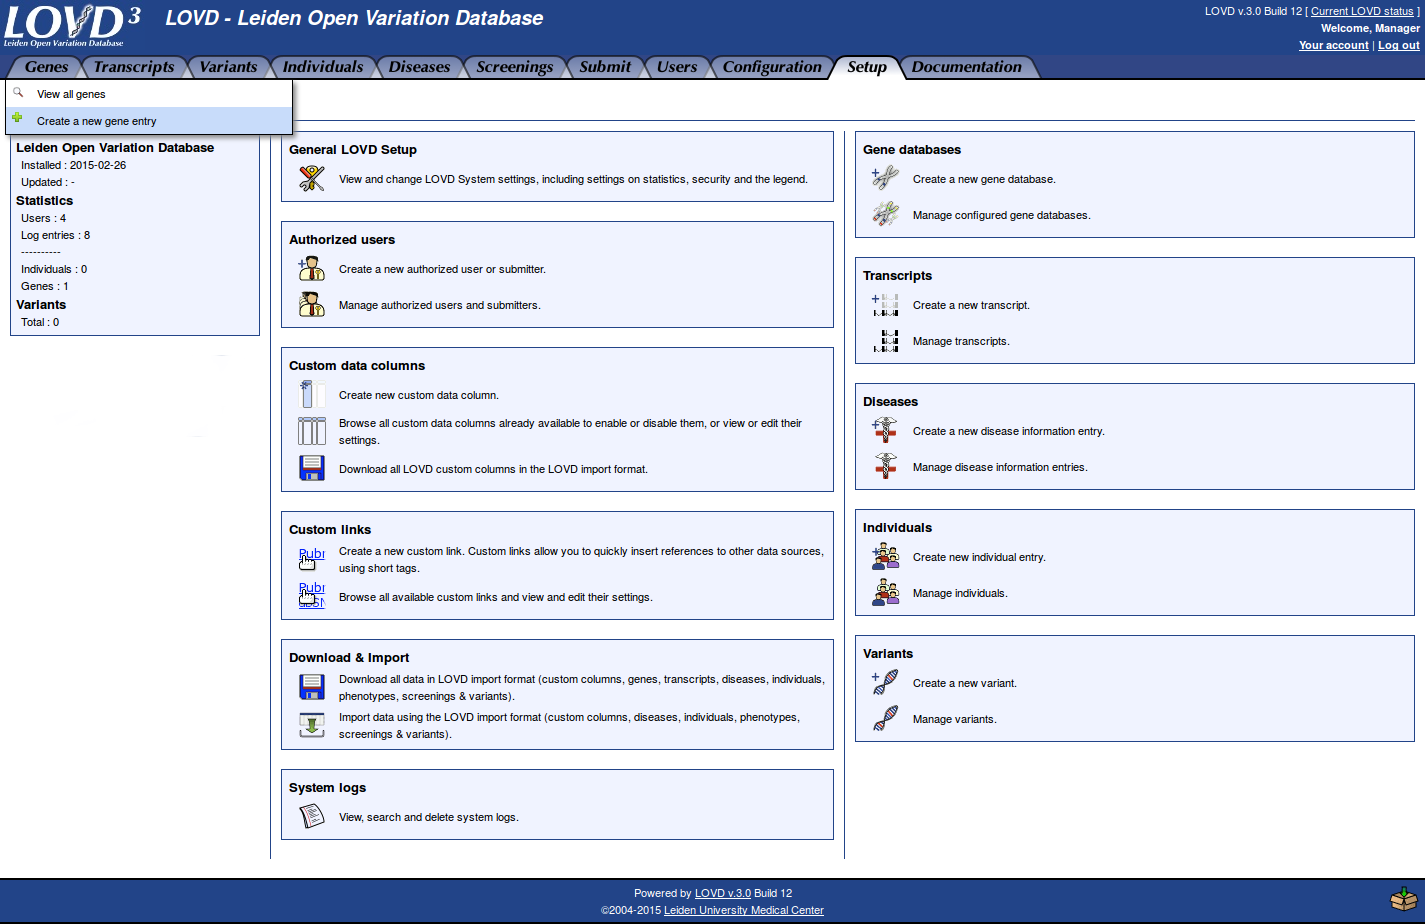
\includegraphics[width=\linewidth]
		   	 {/create_gene/create_gene_I.png}};
		  	\begin{scope}[x={(image.south east)},y={(image.north west)}]
		      \draw[red,ultra thick,rounded corners] (0.005,0.85) rectangle (0.21,0.885);
					\draw[<-, >=latex, \pointercolor, line width=\pointerwidth] (0.21,0.8675) to node[black]{A} (0.31,0.8675);
		      \draw[red,ultra thick,rounded corners] (0.6,0.79) rectangle (0.78,0.85);
					\draw[<-, >=latex, \pointercolor, line width=\pointerwidth] (0.6,0.82) to node[black]{B} (0.5,0.82);
					%\drawgrid %help grid when positioning the boxes and pointers
		  	\end{scope}
			\end{tikzpicture}}
	  \caption{Create a new gene.
	  You can do that via the ``Create a new gene entry'' link from the Genes menu tab drop down menu (A). \newline
	  You can also do that from the Setup area and click the ``Create a new gene database'' link listed under
			``Gene databases'' (B).}
		\label{fig:create_gene_I}
  \end{shaded}
\end{figure}

\begin{figure}[ht]
  \begin{shaded}
		\frame{
			\begin{tikzpicture}
		  	\node[anchor=south west,inner sep=0] (image) at (0,0) {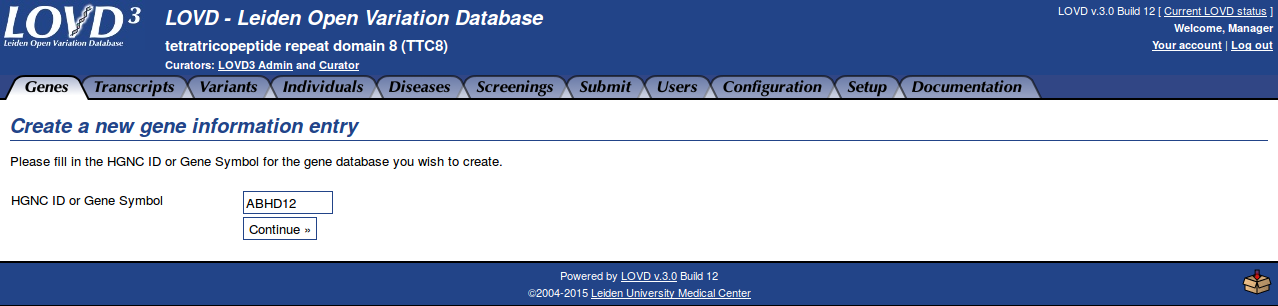
\includegraphics[width=\linewidth]
		   	 {/create_gene/create_gene_ABHD12_I.png}};
			\end{tikzpicture}}
	  \caption{Insert the HGNC gene symbol.\newline
	  You can find the symbol at the HGNC (http://www.genenames.org/) or at the NCBI entrez gene.\newline
		In our example we will use the gene symbol ABHD12. Hereafter, press ``Continue''.}
  \label{fig:create_gene_ABHD12}
  \end{shaded}
\end{figure}

\begin{figure}[ht]
  \begin{shaded}
		\frame{
			\begin{tikzpicture}
				\node[anchor=south west,inner sep=0] (image) at (0,0) {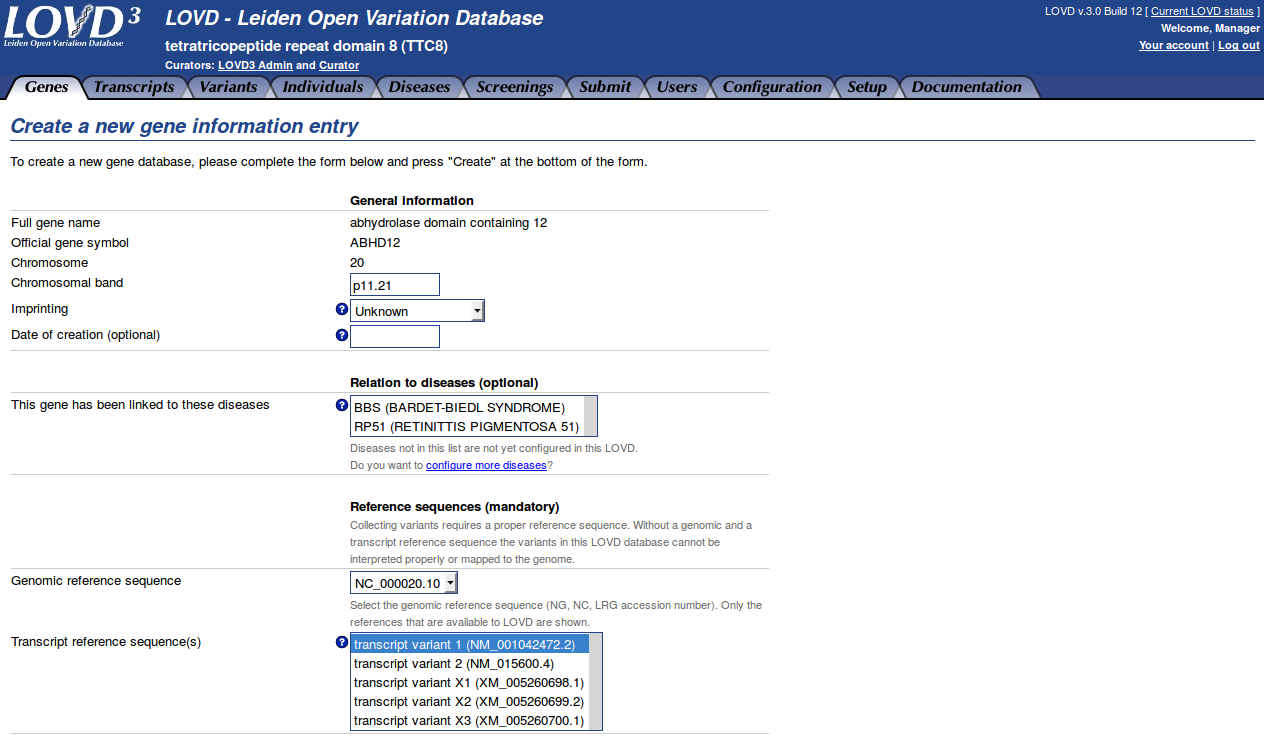
\includegraphics[width=\linewidth]
			 	 {/create_gene/create_gene_ABHD12_II.png}};
				\begin{scope}[x={(image.south east)},y={(image.north west)}]
			    \draw[red,ultra thick,rounded corners] (0.26,0.4) rectangle (0.48,0.5);
					\draw[<-, >=latex, \pointercolor, line width=\pointerwidth] (0.48,0.45) to node[black]{A} (0.58,0.45);
			    \draw[red,ultra thick,rounded corners] (0.26,0.19) rectangle (0.37,0.24);
					\draw[<-, >=latex, \pointercolor, line width=\pointerwidth] (0.37,0.225) to node[black]{B} (0.47,0.225);
			    \draw[red,ultra thick,rounded corners] (0.26,0.005) rectangle (0.48,0.18);
					\draw[<-, >=latex, \pointercolor, line width=\pointerwidth] (0.48,0.08975) to node[black]{C} (0.58,0.08975);
					%\drawgrid %help grid when positioning the boxes and pointers
				\end{scope}
			\end{tikzpicture}}
		\caption{You can link a Disease to this gene (A). 
		But the genes listed here are from previous exercises and are not linked to our current gene. 
		We could create diseases from here, see figure \ref{curate_gene_fig:edit_gene_III} in course manual ``Curate gene 		 variant database'' how.
		For now, do not select any disease, we will create a new disease later.\newline
		For ``Genomic reference sequence'', select ``NC\_000020.10'' (B) and for ``Transcript reference sequences'',
		 select ``NM\_001042472.2'' (C).}
		\label{fig:create_gene_ABHD12_II}
  \end{shaded}
\end{figure}

\begin{figure}[ht]
  \begin{shaded}
  	\frame{
			\begin{tikzpicture}
				\node[anchor=south west,inner sep=0] (image) at (0,0) {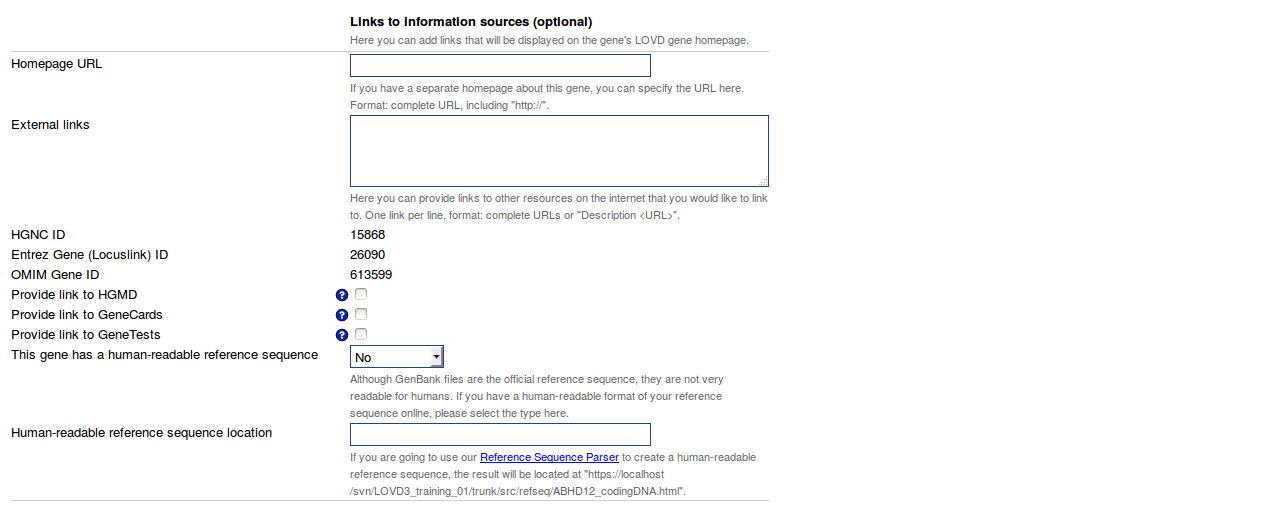
\includegraphics[width=\linewidth]
			 	 {/create_gene/create_gene_ABHD12_III.png}};
				\begin{scope}[x={(image.south east)},y={(image.north west)}]
			    %\draw[red,ultra thick,rounded corners] (0.24,0.43) rectangle (0.38,0.5);
					%\draw[<-, >=latex, \pointercolor, line width=\pointerwidth] (0.38,0.47) to node[black]{A} (0.48,0.47);
					%\drawgrid %help grid when positioning the boxes and pointers
				\end{scope}
			\end{tikzpicture}}
		\caption{You can provide links to other resources on the internet that you would like to link to.}
		\label{fig:create_gene_ABHD12_III}
  \end{shaded}
\end{figure}

\begin{figure}[ht]
  \begin{shaded}
		\frame{
	 		\begin{tikzpicture}
				\node[anchor=south west,inner sep=0] (image) at (0,0) {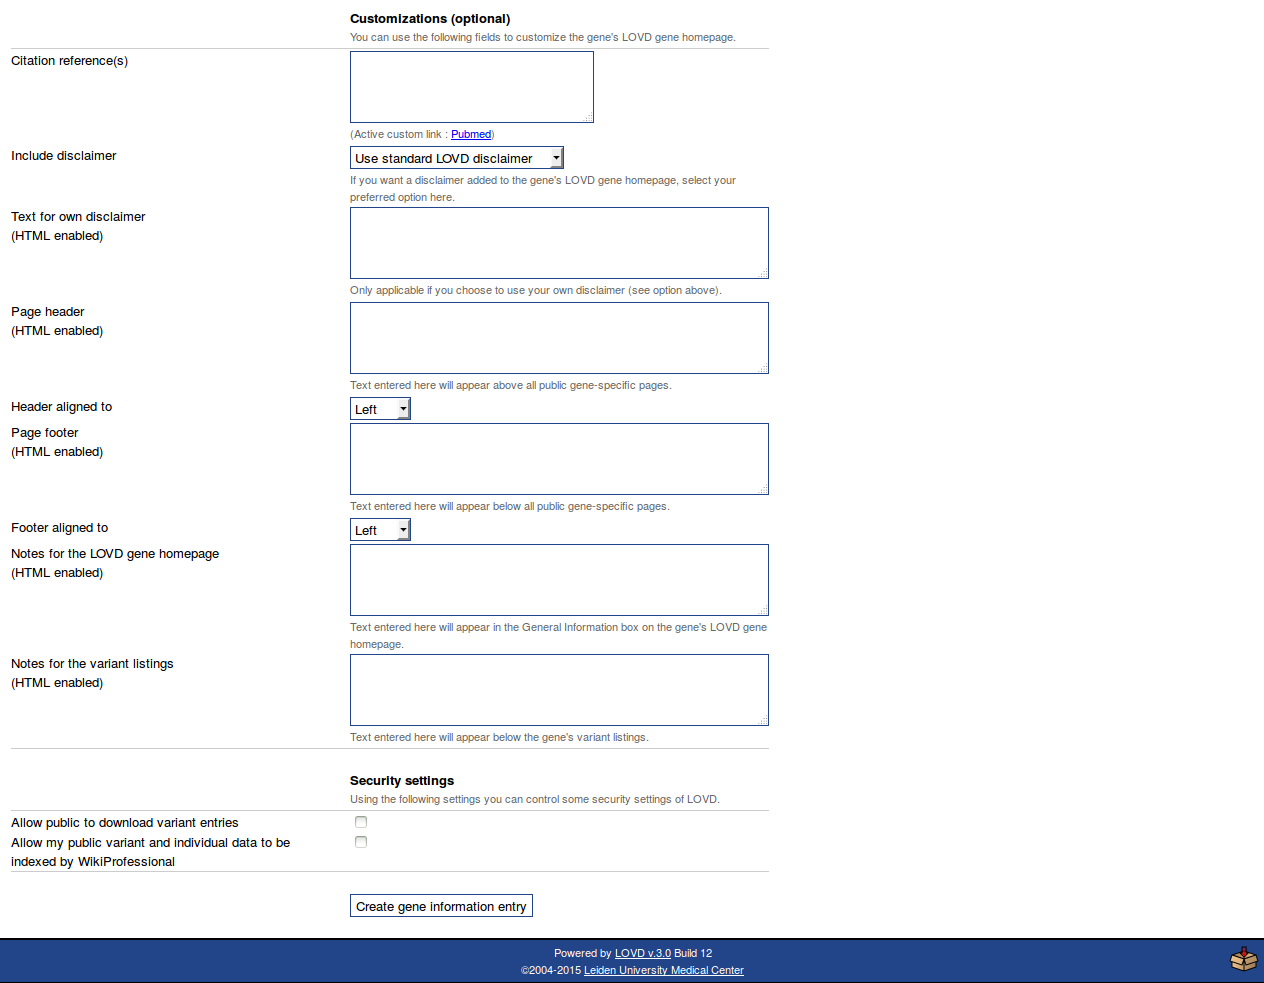
\includegraphics[width=\linewidth]
			 	 {/create_gene/create_gene_ABHD12_IV.png}};
				\begin{scope}[x={(image.south east)},y={(image.north west)}]
			    %\draw[red,ultra thick,rounded corners] (0.24,0.43) rectangle (0.38,0.5);
					%\draw[<-, >=latex, \pointercolor, line width=\pointerwidth] (0.38,0.47) to node[black]{A} (0.48,0.47);
					%\drawgrid %help grid when positioning the boxes and pointers
				\end{scope}
			\end{tikzpicture}}
		\caption{You can add a disclaimer, page header or page footer to the gene's LOVD gene homepage.
		Click ``Create gene information entry'' when you are ready. \newline
		Hereafter you are redirected to ``Authorize curators for the gene''.
		We will come back later on this subject in chapter ``\nameref{chap:create_manage_users}''.
		For now, click ``Cancel''.}
		\label{fig:create_gene_ABHD12_IV}
  \end{shaded}
\end{figure}










\chapter{Creating a disease}
The objective of this chapter is:
\begin{enumerate}
	\item 
	Create a new disease and link this disease to our gene.
\end{enumerate}

\begin{figure}[ht]
  \begin{shaded}
		\frame{
	 		\begin{tikzpicture}
				\node[anchor=south west,inner sep=0] (image) at (0,0) {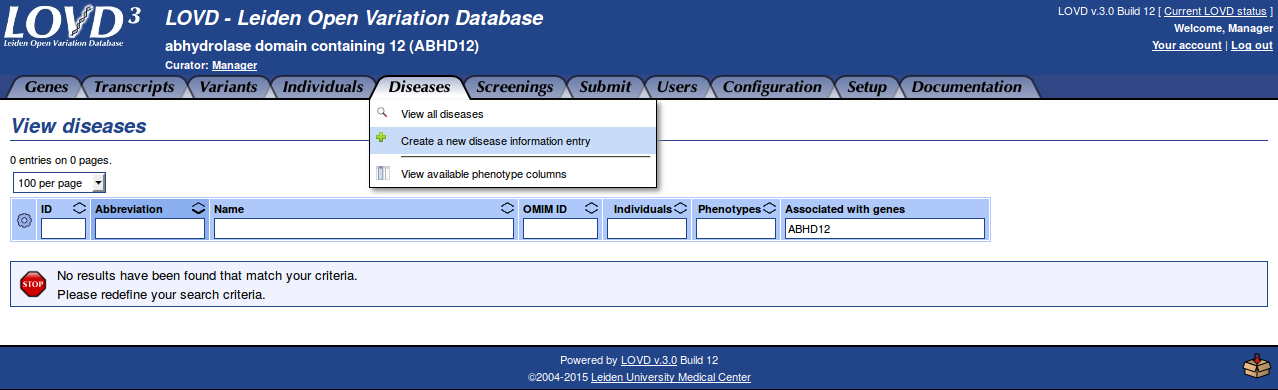
\includegraphics[width=\linewidth]
			 	 {/create_gene/create_disease_PHARC_I.png}};
				\begin{scope}[x={(image.south east)},y={(image.north west)}]
			    %\draw[red,ultra thick,rounded corners] (0.26,0.38) rectangle (0.49,0.6);
					%\draw[<-, >=latex, \pointercolor, line width=\pointerwidth] (0.49,0.49) to node[black]{A} (0.59,0.49);
			    %\draw[red,ultra thick,rounded corners] (0.26,0.22) rectangle (0.49,0.34);
					%\draw[<-, >=latex, \pointercolor, line width=\pointerwidth] (0.49,0.27) to node[black]{B} (0.59,0.27);
					%\drawgrid %help grid when positioning the boxes and pointers
				\end{scope}
			\end{tikzpicture}}
		\caption{To create a new disease, click ``Create a new disease information entry'' from the Disease menu tab.}
		\label{fig:create_disease_PHARC_I}
  \end{shaded}
\end{figure}

\begin{figure}[ht]
  \begin{shaded}
		\frame{
	 		\begin{tikzpicture}
				\node[anchor=south west,inner sep=0] (image) at (0,0) {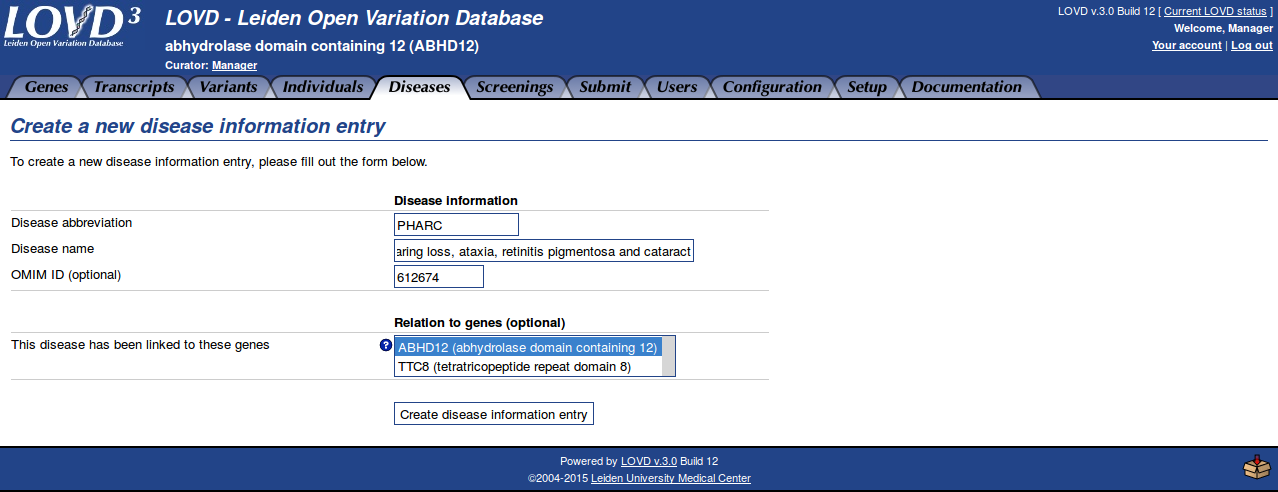
\includegraphics[width=\linewidth]
			 	 {/create_gene/create_disease_PHARC_II.png}};
				\begin{scope}[x={(image.south east)},y={(image.north west)}]
			    \draw[red,ultra thick,rounded corners] (0.29,0.39) rectangle (0.55,0.61);
					\draw[<-, >=latex, \pointercolor, line width=\pointerwidth] (0.55,0.5) to node[black]{A} (0.65,0.5);
			    \draw[red,ultra thick,rounded corners] (0.31,0.22) rectangle (0.55,0.36);
					\draw[<-, >=latex, \pointercolor, line width=\pointerwidth] (0.55,0.29) to node[black]{B} (0.65,0.29);
			    \draw[red,ultra thick,rounded corners] (0.29,0.28) rectangle (0.31,0.33);
					\draw[<-, >=latex, \pointercolor, line width=\pointerwidth] (0.29,0.305) to node[black]{C} (0.19,0.305);
					%\drawgrid %help grid when positioning the boxes and pointers
				\end{scope}
			\end{tikzpicture}}
		\caption{Give disease abbreviation, name and OMIM ID (A). \newline
		You can make a relation with a gene by selecting one or more genes (B).
		See help text for how to select multiple genes (C).
		In our example, we select ABHD12 and click ``Create disease information entry''.}
		\label{fig:create_disease_PHARC_II}
  \end{shaded}
\end{figure}










\chapter{Creating and managing columns}
The objective of this chapter is:
\begin{enumerate}
	\item 
	Create a new custom column.
	\item 
	Manage the custom column.
\end{enumerate}
To start this chapter:
\begin{itemize}
	\item 
	See chapter ``\nameref{curate_gene_edit_columns_legends}'' in course manual ``Curate gene variant \\
		database'' for some additional exercises on custom columns.
\end{itemize}

\section{Create new custom columns}
\begin{figure}[ht]
  \begin{shaded}
		\frame{
				\begin{tikzpicture}
					\node[anchor=south west,inner sep=0] (image) at (0,0) {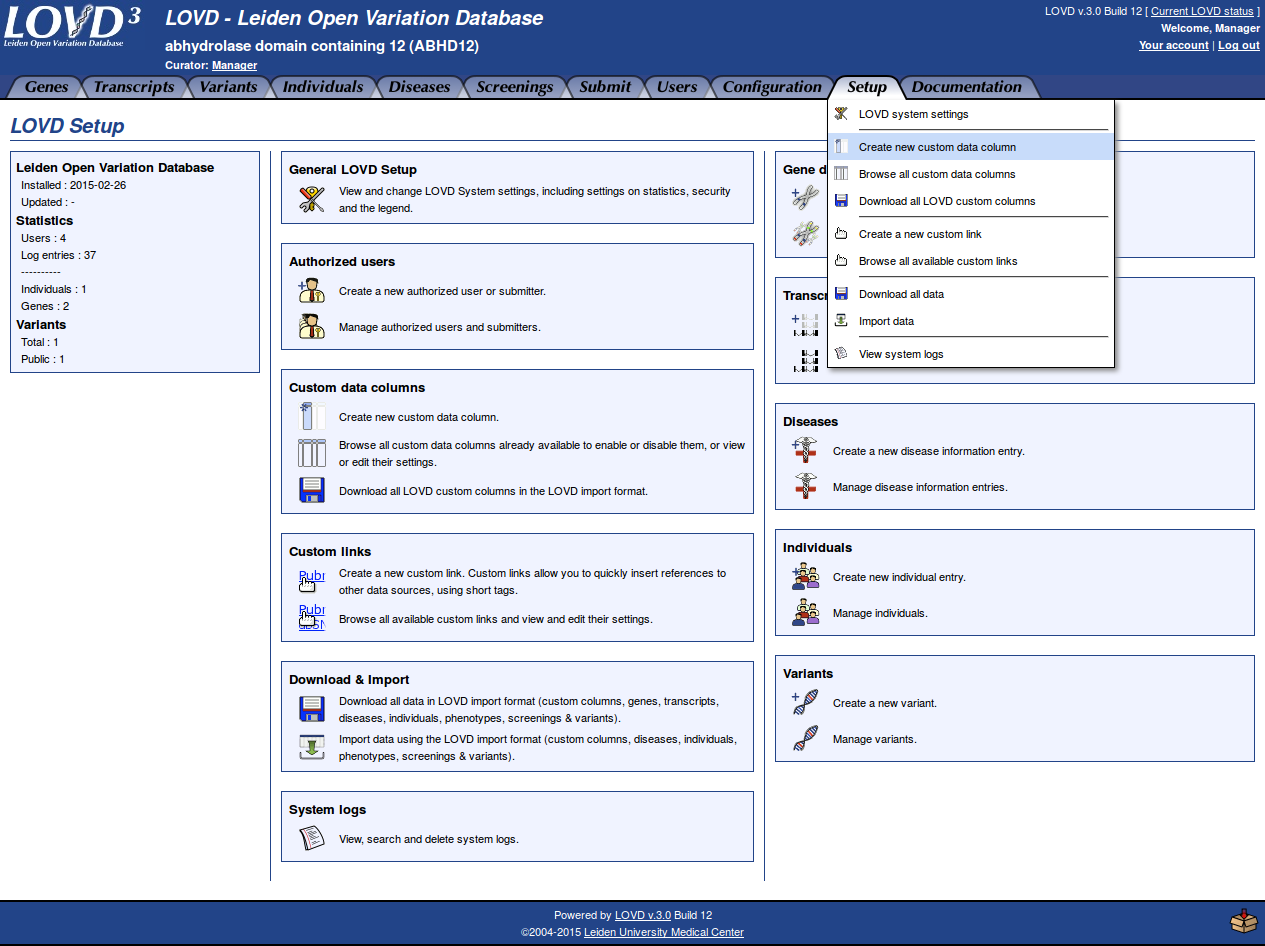
\includegraphics[width=\linewidth]
				 	 {/create_gene/create_column_I.png}};
					\begin{scope}[x={(image.south east)},y={(image.north west)}]
				    \draw[red,ultra thick,rounded corners] (0.65,0.83) rectangle (0.82,0.86);
						\draw[<-, >=latex, \pointercolor, line width=\pointerwidth] (0.82,0.845) to node[black]{A} (0.92,0.845);
				    \draw[red,ultra thick,rounded corners] (0.22,0.54) rectangle (0.42,0.605);
						\draw[<-, >=latex, \pointercolor, line width=\pointerwidth] (0.42,0.57) to node[black]{B} (0.52,0.57);
						%\drawgrid %help grid when positioning the boxes and pointers
					\end{scope}
				\end{tikzpicture}}
		\caption{You can create a new column via the ``Create new custom data column'' link from the Setup drop down
		 menu tab (A), or you can click ``Create new custom data column'' from the Setup area (B).}
		\label{fig:create_column_I}
  \end{shaded}
\end{figure}

\begin{figure}[ht]
  \begin{shaded}
			\frame{
				\begin{tikzpicture}
					\node[anchor=south west,inner sep=0] (image) at (0,0) {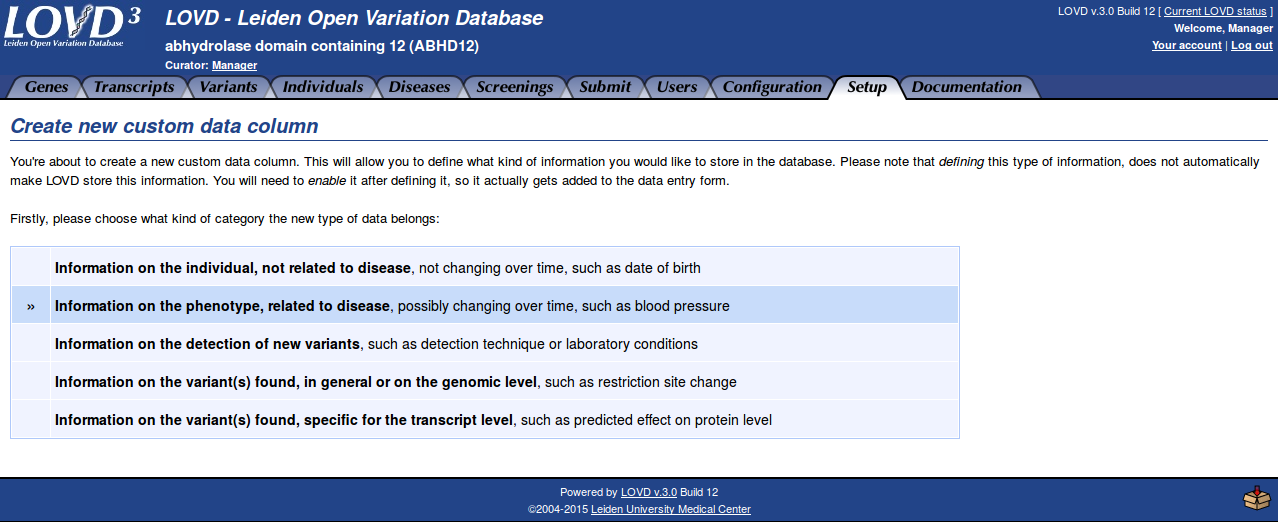
\includegraphics[width=\linewidth]
				 	 {/create_gene/create_column_II.png}};
					\begin{scope}[x={(image.south east)},y={(image.north west)}]
				    %\draw[red,ultra thick,rounded corners] (0.01,0.38) rectangle (0.6,0.46);
						%\draw[<-, >=latex, \pointercolor, line width=\pointerwidth] (0.6,0.42) to node[black]{C} (0.7,0.42);
						%\drawgrid %help grid when positioning the boxes and pointers
					\end{scope}
				\end{tikzpicture}}
		\caption{Select the category to which the new type of data belongs to. 
		In our example we will add a new column ``Neurography and EMG'' (see table 1 in Fiskerstrand et al., 2010).
		This is a phenotype field related to disease, so select ``Information on the phenotype, related to disease''.}
		\label{fig:create_column_II}
  \end{shaded}
\end{figure}

\begin{figure}[ht]
  \begin{shaded}
		\frame{
			\begin{tikzpicture}
				\node[anchor=south west,inner sep=0] (image) at (0,0) {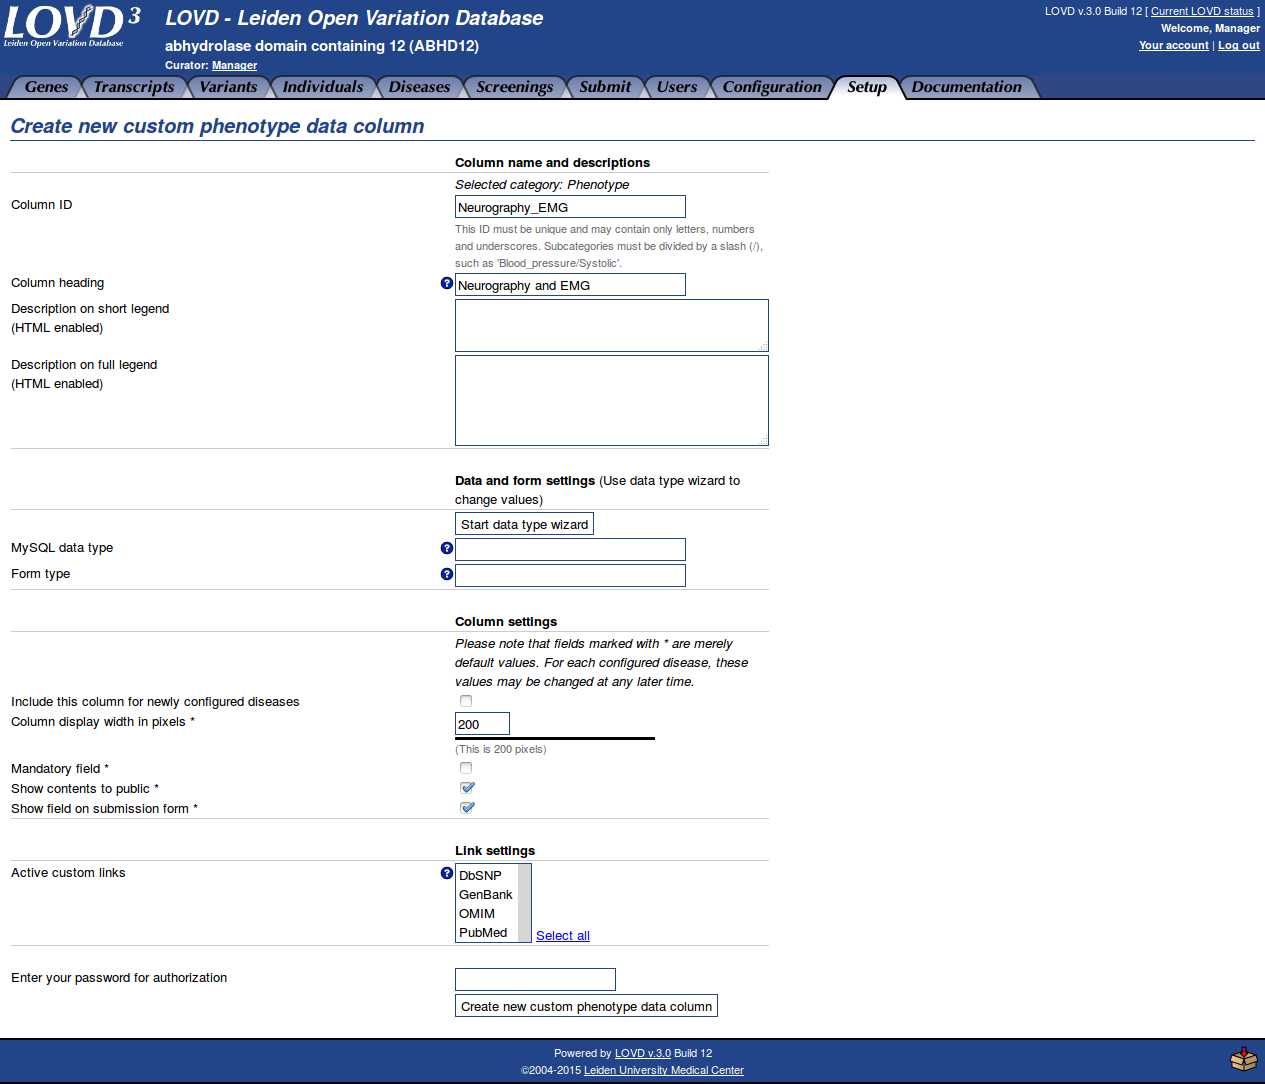
\includegraphics[width=\linewidth]
			 	 {/create_gene/create_column_III.png}};
				\begin{scope}[x={(image.south east)},y={(image.north west)}]
				  \draw[red,ultra thick,rounded corners] (0.34,0.58) rectangle (0.62,0.87);
					\draw[<-, >=latex, \pointercolor, line width=\pointerwidth] (0.62,0.725) to node[black]{A} (0.72,0.725);
				  \draw[red,ultra thick,rounded corners] (0.34,0.505) rectangle (0.6,0.57);
					\draw[<-, >=latex, \pointercolor, line width=\pointerwidth] (0.6,0.5375) to node[black]{B} (0.7,0.5375);
				  \draw[red,ultra thick,rounded corners] (0.34,0.45) rectangle (0.55,0.505);
					\draw[<-, >=latex, \pointercolor, line width=\pointerwidth] (0.55,0.4775) to node[black]{C} (0.65,0.4775);
					%\drawgrid %help grid when positioning the boxes and pointers
				\end{scope}
			\end{tikzpicture}}
		\caption{Fill the fields under section ``Column name and description'': Column ID, Column heading, Description on
		 short legend and Description on full legend (A).\newline
		Then press ``Start data type wizard'' under section ``Data and form settings'' (B). 
		This will open a pop-up screen where you can determine the data type for your new column.
		The results of the data type wizard are saved in the fields ``MySQL data type'' and ``Form type'' (C).\newline
		Only if you really know what you're doing, you can edit ``MySQL data type'' and ``Form type'' directly (C).}
		\label{fig:create_column_III}
  \end{shaded}
\end{figure}

\begin{figure}[ht]
  \begin{shaded}
		\frame{
			\begin{tikzpicture}
				\node[anchor=south west,inner sep=0] (image) at (0,0) {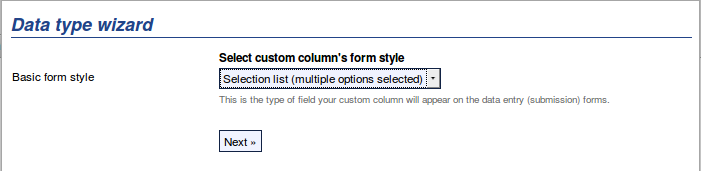
\includegraphics[width=\linewidth]
			 	 {/create_gene/create_column_IV.png}};
				\begin{scope}[x={(image.south east)},y={(image.north west)}]
				  \draw[red,ultra thick,rounded corners] (0.3,0.46) rectangle (0.64,0.71);
					\draw[<-, >=latex, \pointercolor, line width=\pointerwidth] (0.64,0.585) to node[black]{A} (0.74,0.585);
					%\drawgrid %help grid when positioning the boxes and pointers
				\end{scope}
			\end{tikzpicture}}
		\vskip 3mm
		\frame{
			\begin{tikzpicture}
				\node[anchor=south west,inner sep=0] (image) at (0,0) {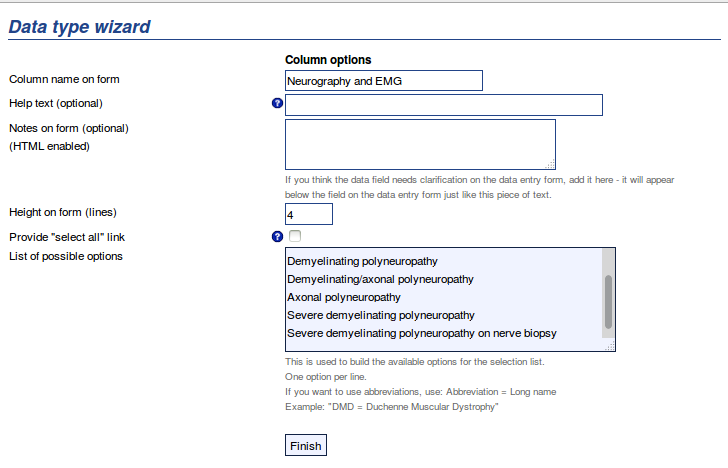
\includegraphics[width=\linewidth]
			 	 {/create_gene/create_column_V.png}};
				\begin{scope}[x={(image.south east)},y={(image.north west)}]
				  \draw[red,ultra thick,rounded corners] (0.38,0.24) rectangle (0.86,0.48);
					\draw[<-, >=latex, \pointercolor, line width=\pointerwidth] (0.38,0.36) to node[black]{B} (0.28,0.36);
					%\drawgrid %help grid when positioning the boxes and pointers
				\end{scope}
			\end{tikzpicture}}
		\caption{Here you may choose between the following type of input fields (A):
	 	Text/numeric, Integer, Decimal, Large multi-row textual, Drop down list (1 option selected), Selection list
	 	 (multiple selection), date and On/Off checkbox.
		In our example we use ``Selection list (multiple options selected)''.
		Press ``Next'' when you're ready.\newline
		In the second data type wizard form you can list the options (B). 
		Use the data from the ``Neurography and EMG'' (see table 1 in Fiskerstrand et al 2010) column.
		Put each option on a new line and press ``Finish'' when you are ready.}
		\label{fig:create_column_IV}
  \end{shaded}
\end{figure}

\begin{figure}[ht]
  \begin{shaded}
		\frame{
			\begin{tikzpicture}
				\node[anchor=south west,inner sep=0] (image) at (0,0) {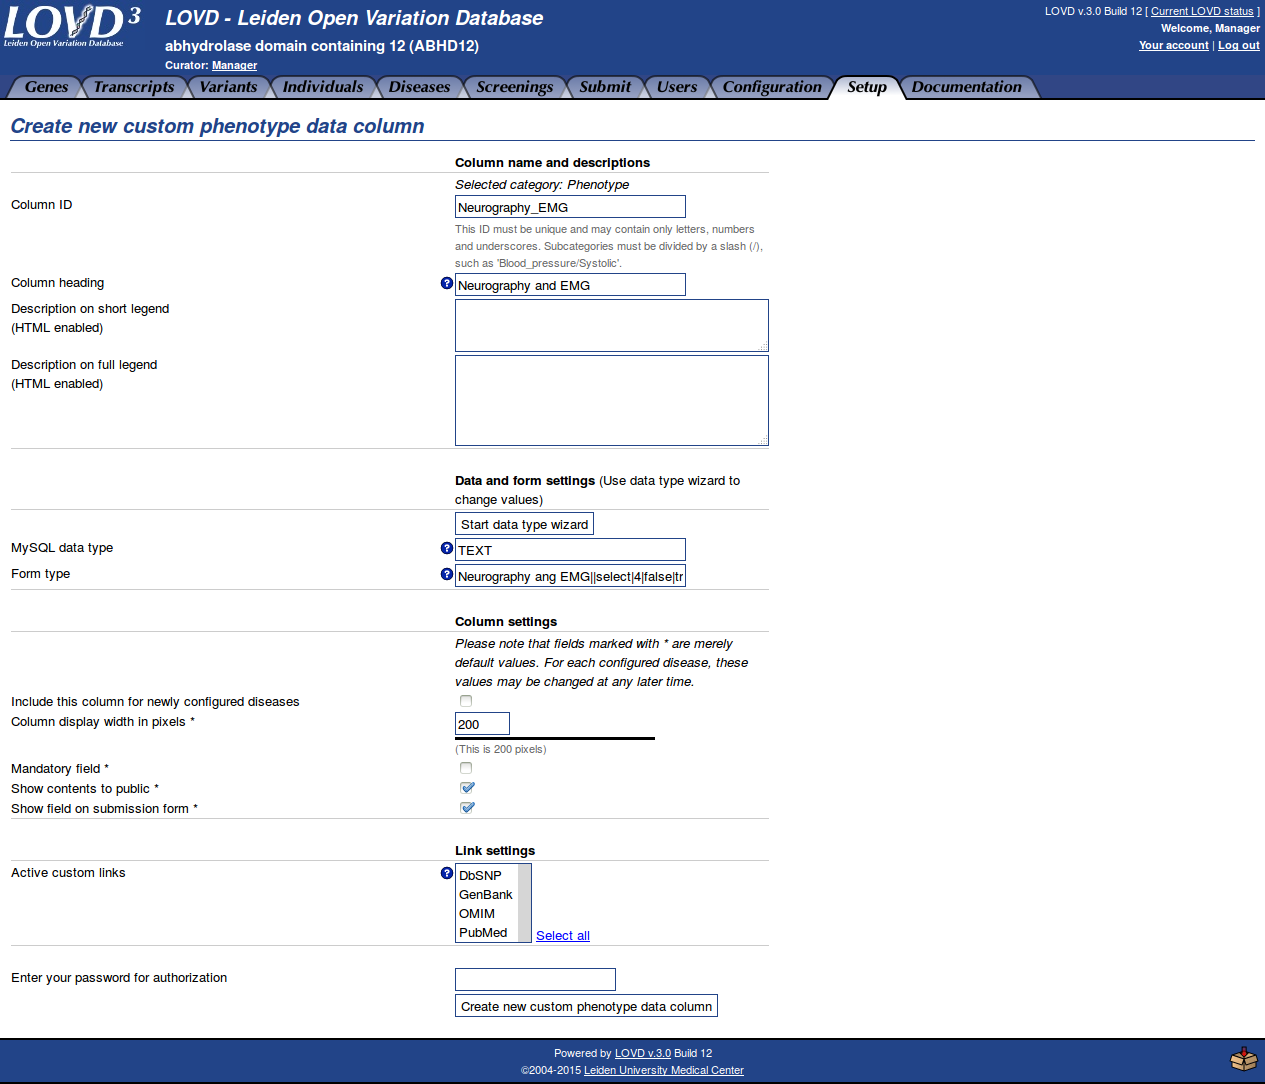
\includegraphics[width=\linewidth]
			 	 {/create_gene/create_column_VI.png}};
				\begin{scope}[x={(image.south east)},y={(image.north west)}]
				  \draw[red,ultra thick,rounded corners] (0.345,0.455) rectangle (0.58,0.51);
					\draw[<-, >=latex, \pointercolor, line width=\pointerwidth] (0.58,0.4825) to node[black]{A} (0.68,0.4825);
				  \draw[red,ultra thick,rounded corners] (0.34,0.25) rectangle (0.64,0.44);
					\draw[<-, >=latex, \pointercolor, line width=\pointerwidth] (0.64,0.345) to node[black]{B} (0.74,0.345);
				  \draw[red,ultra thick,rounded corners] (0.345,0.12) rectangle (0.48,0.23);
					\draw[<-, >=latex, \pointercolor, line width=\pointerwidth] (0.48,0.175) to node[black]{C} (0.58,0.175);
				  \draw[red,ultra thick,rounded corners] (0.345,0.05) rectangle (0.6,0.115);
					\draw[<-, >=latex, \pointercolor, line width=\pointerwidth] (0.6,0.0825) to node[black]{D} (0.7,0.0825);
					%\drawgrid %help grid when positioning the boxes and pointers
				\end{scope}
			\end{tikzpicture}}
		\caption{The data type wizard will automatically fill the fields ``MySQL data type'' and ``Form type'' (A). 
		Choose column settings (B), specific custom links for this column (C), confirm with your password and press 
			``Create new custom phenotype data column'' (D) when you are ready.}
    \label{fig:create_column_VI}
  \end{shaded}
\end{figure}
\clearpage





\section{Managing custom columns}
\begin{figure}[ht]
  \begin{shaded}
		\frame{
			\begin{tikzpicture}
				\node[anchor=south west,inner sep=0] (image) at (0,0) {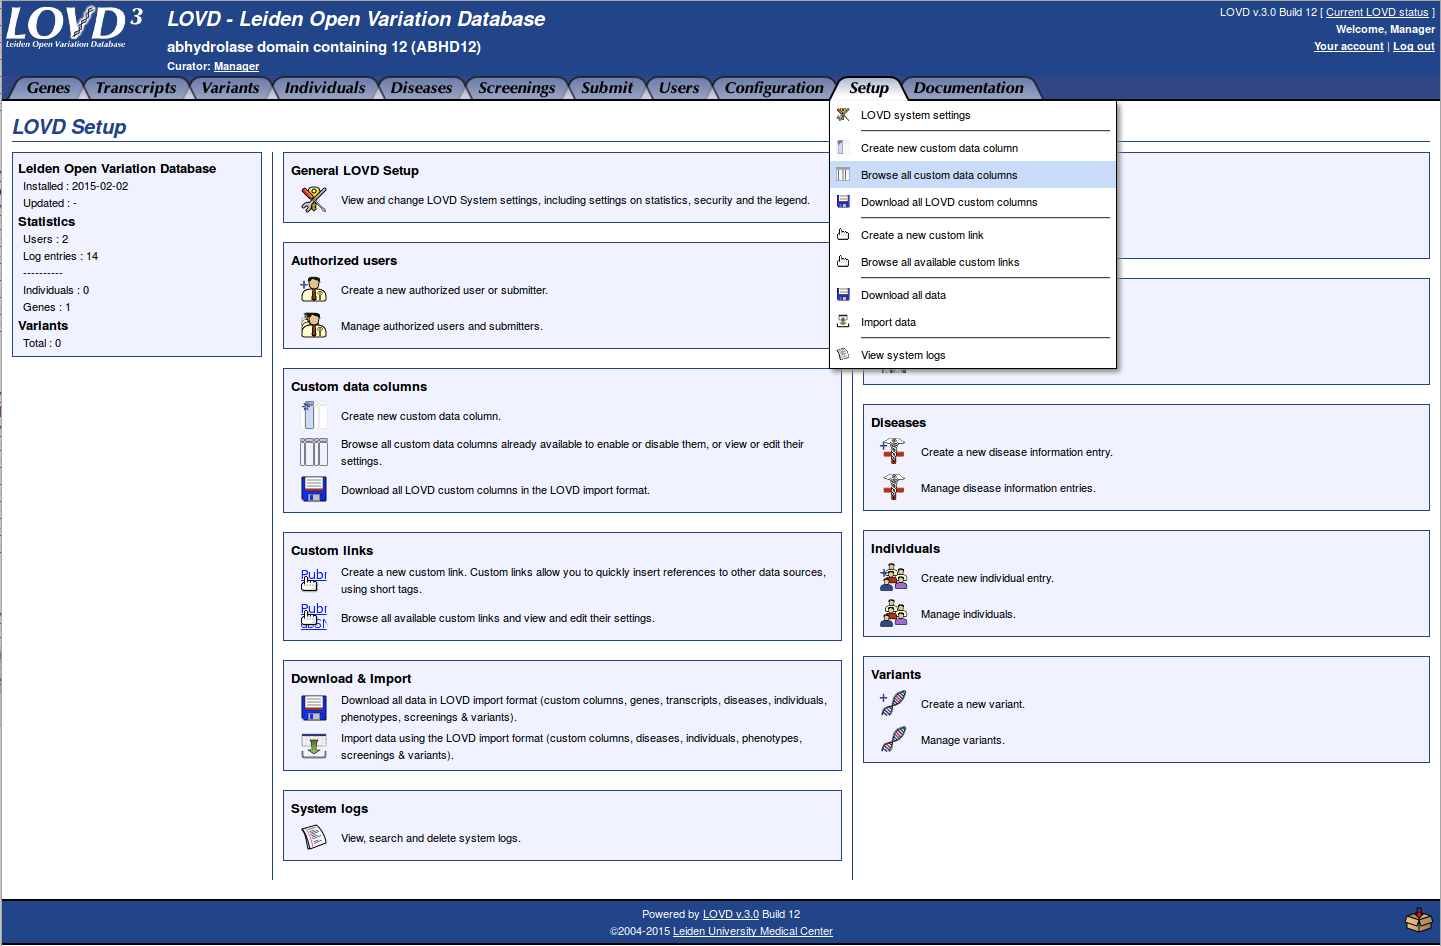
\includegraphics[width=\linewidth]
			 	 {/create_gene/manage_column_I.png}};
				\begin{scope}[x={(image.south east)},y={(image.north west)}]
				  \draw[red,ultra thick,rounded corners] (0.57,0.795) rectangle (0.73,0.835);
					\draw[<-, >=latex, \pointercolor, line width=\pointerwidth] (0.73,0.815) to node[black]{A} (0.83,0.815);
				  \draw[red,ultra thick,rounded corners] (0.195,0.5) rectangle (0.58,0.55);
					\draw[<-, >=latex, \pointercolor, line width=\pointerwidth] (0.58,0.525) to node[black]{B} (0.68,0.525);
					%\drawgrid %help grid when positioning the boxes and pointers
				\end{scope}
			\end{tikzpicture}}
		\caption{You can browse all custom columns via the ``Browse all custom data columns'' link from the Setup
		drop down menu tab (A), or you can select ``Browse all custom data columns (...)'' from the Setup area (B).}
  	\label{fig:manage_column_I}
  \end{shaded}
\end{figure}

\begin{figure}[ht]
  \begin{shaded}
		\frame{
			\begin{tikzpicture}
				\node[anchor=south west,inner sep=0] (image) at (0,0) {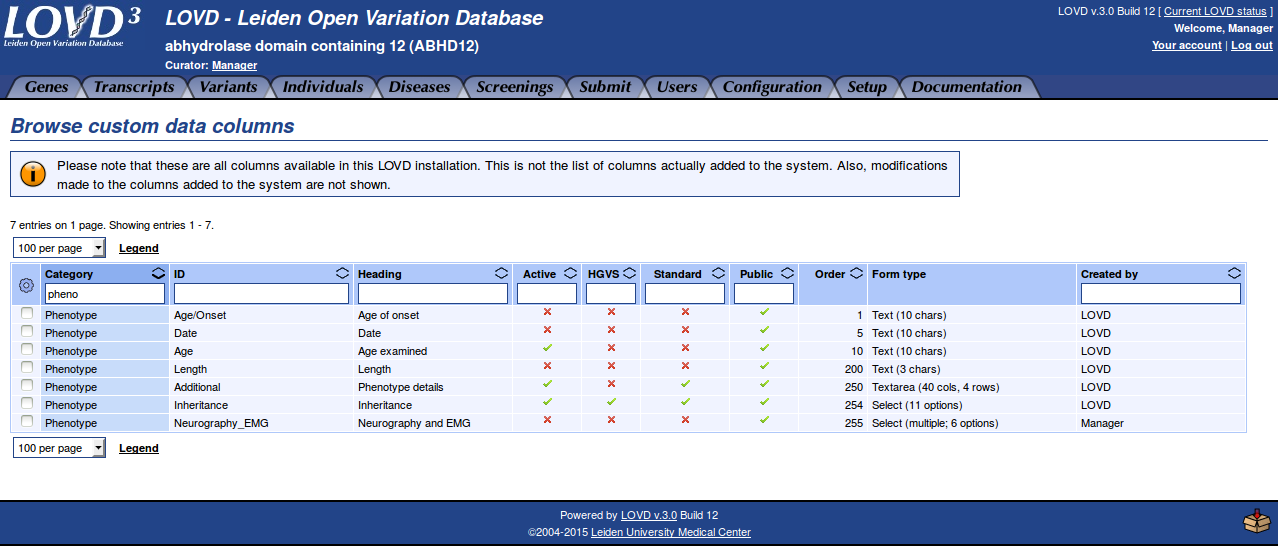
\includegraphics[width=\linewidth]
			 	 {/create_gene/manage_column_II.png}};
				\begin{scope}[x={(image.south east)},y={(image.north west)}]
				  \draw[red,ultra thick,rounded corners] (0.03,0.44) rectangle (0.63,0.52);
					\draw[<-, >=latex, \pointercolor, line width=\pointerwidth] (0.63,0.48) to node[black]{A} (0.73,0.48);
				  \draw[red,ultra thick,rounded corners] (0.01,0.44) rectangle (0.03,0.52);
					\draw[<-, >=latex, \pointercolor, line width=\pointerwidth] (0.02,0.52) to node[black]{B} (0.02,0.76);
				  \draw[red,ultra thick,rounded corners] (0.03,0.2) rectangle (0.63,0.25);
					\draw[<-, >=latex, \pointercolor, line width=\pointerwidth] (0.63,0.225) to node[black]{C} (0.73,0.225);
					%\drawgrid %help grid when positioning the boxes and pointers
				\end{scope}
			\end{tikzpicture}}
		\caption{If you want to display custom columns only applicable for phenotype, 
		 you can use the headers as a filter (A). 
		Or you can use the menu on the left (B) and select ``Show only Phenotype columns''.
		Look for your newly created custom column (C).
		You can see that your new custom column is not active yet.\newline
		Click anywhere on the row to go to the details of your custom column. }
  	\label{fig:manage_column_II}
  \end{shaded}
\end{figure}

\begin{figure}[ht]
  \begin{shaded}
  	\frame{
			\begin{tikzpicture}
				\node[anchor=south west,inner sep=0] (image) at (0,0) {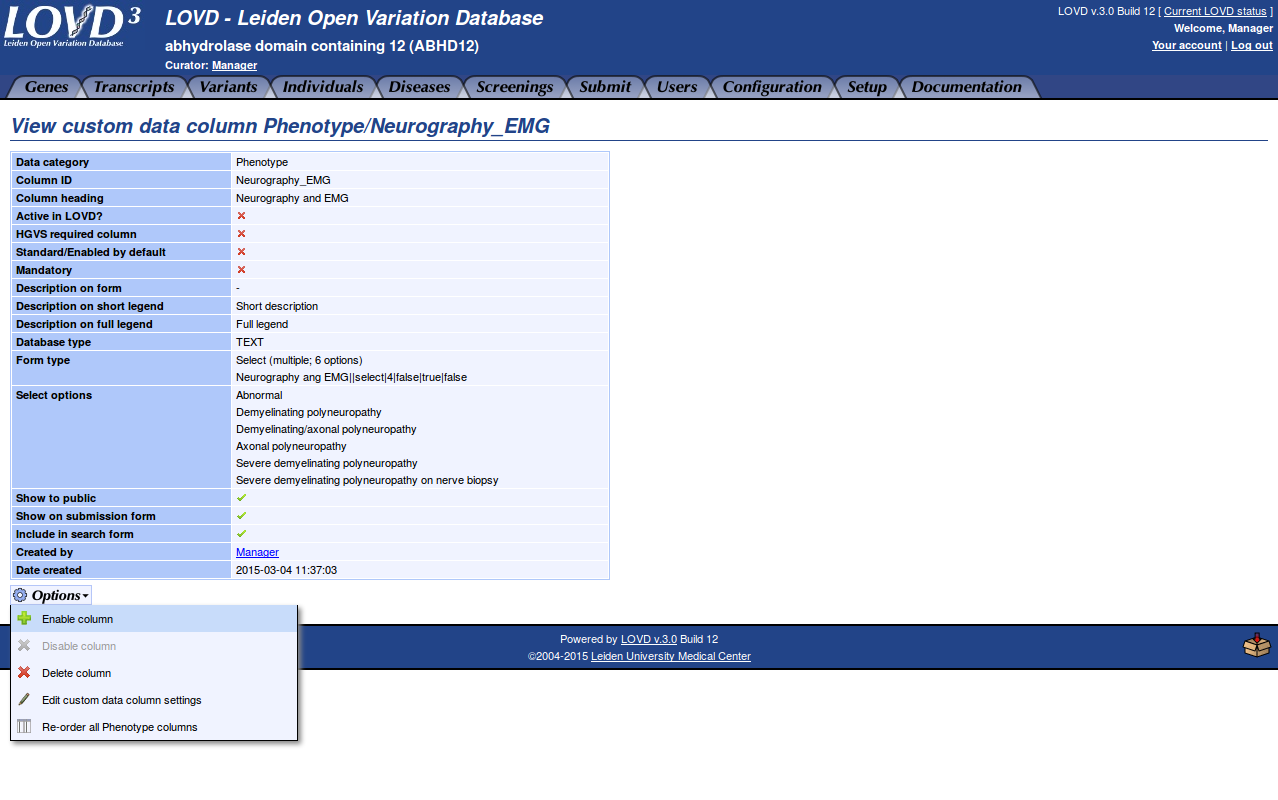
\includegraphics[width=\linewidth]
			 	 {/create_gene/manage_column_III.png}};
				\begin{scope}[x={(image.south east)},y={(image.north west)}]
				  \draw[red,ultra thick,rounded corners] (0.006,0.21) rectangle (0.15,0.24);
					\draw[<-, >=latex, \pointercolor, line width=\pointerwidth] (0.15,0.225) to node[black]{} (0.25,0.225);
					%\drawgrid %help grid when positioning the boxes and pointers
				\end{scope}
			\end{tikzpicture}}
		\caption{Click the Options drop down menu and click ``Enable column''. 
		If you click ``Edit custom data column settings'', you will go to the form ``Edit custom data column''. 
		This form is similar to the form ``Create custom data column'', see figure \ref{fig:create_column_III}.}
    \label{fig:manage_column_III}
  \end{shaded}
\end{figure}

\begin{figure}[ht]
  \begin{shaded}
  	\frame{
			\begin{tikzpicture}
				\node[anchor=south west,inner sep=0] (image) at (0,0) {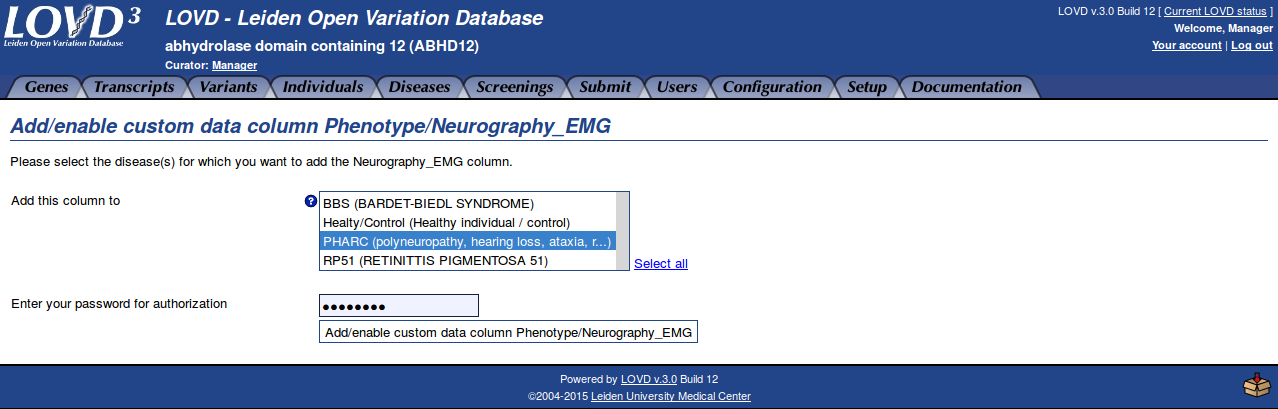
\includegraphics[width=\linewidth]
			 	 {/create_gene/manage_column_IV.png}};
				\begin{scope}[x={(image.south east)},y={(image.north west)}]
				  %\draw[red,ultra thick,rounded corners] (0.006,0.21) rectangle (0.15,0.24);
					%\draw[<-, >=latex, \pointercolor, line width=\pointerwidth] (0.15,0.225) to node[black]{} (0.25,0.225);
					%\drawgrid %help grid when positioning the boxes and pointers
				\end{scope}
			\end{tikzpicture}}
  	\caption{Select to which disease you want to add the custom column, in our example we select PHARC. 
  	You can select multiple diseases, see help text for how to select multiple diseases.\newline
  	Confirm with your password.}
  \label{fig:manage_column_IV}
  \end{shaded}
\end{figure}

\begin{figure}[ht]
  \begin{shaded}
  	\frame{
			\begin{tikzpicture}
				\node[anchor=south west,inner sep=0] (image) at (0,0) {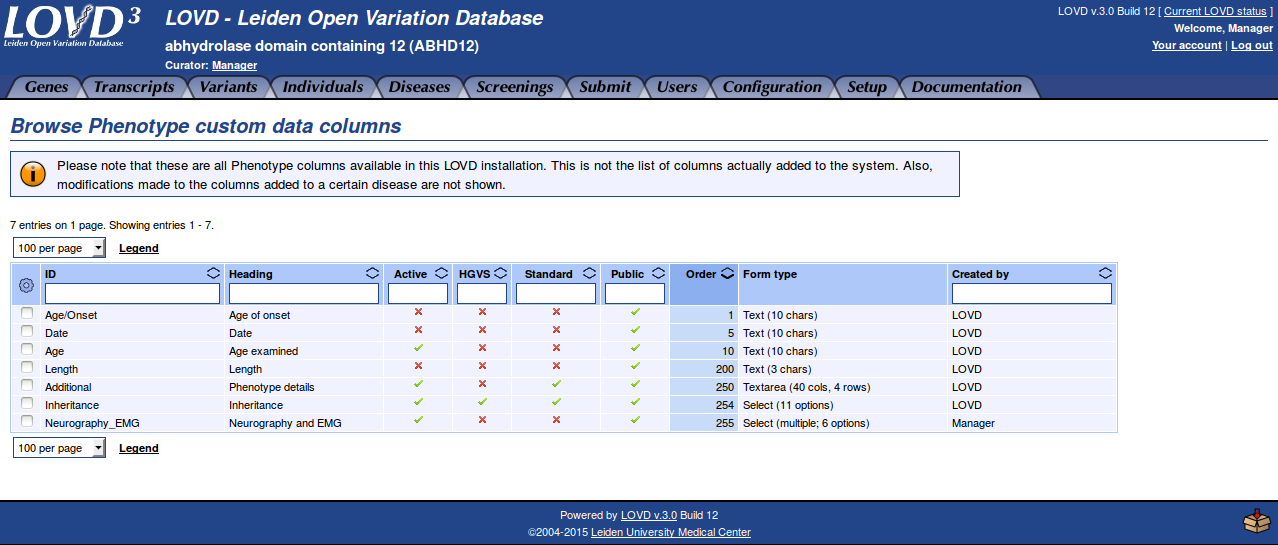
\includegraphics[width=\linewidth]
			 	 {/create_gene/manage_column_V.png}};
				\begin{scope}[x={(image.south east)},y={(image.north west)}]
				  \draw[red,ultra thick,rounded corners] (0.15,0.2) rectangle (0.34,0.25);
					\draw[<-, >=latex, \pointercolor, line width=\pointerwidth] (0.15,0.225) to node[black]{} (0.05,0.225);
					%\drawgrid %help grid when positioning the boxes and pointers
				\end{scope}
			\end{tikzpicture}}
		\caption{In the view ``Browse custom data columns'' you can see that your custom column is now Active (A).\newline
		If you want to change the settings of your custom column go to the ``View custom data column'' page, 
		 see figure \ref{fig:manage_column_III} and click ``Edit custom data column settings''.}
	  \label{fig:manage_column_V}
  \end{shaded}
\end{figure}











\chapter{Creating a custom link}
The objective of this chapter is:
\begin{enumerate}
	\item 
	Create new custom link.
\end{enumerate}

\begin{figure}[ht]
  \begin{shaded}
  	\frame{
			\begin{tikzpicture}
				\node[anchor=south west,inner sep=0] (image) at (0,0) {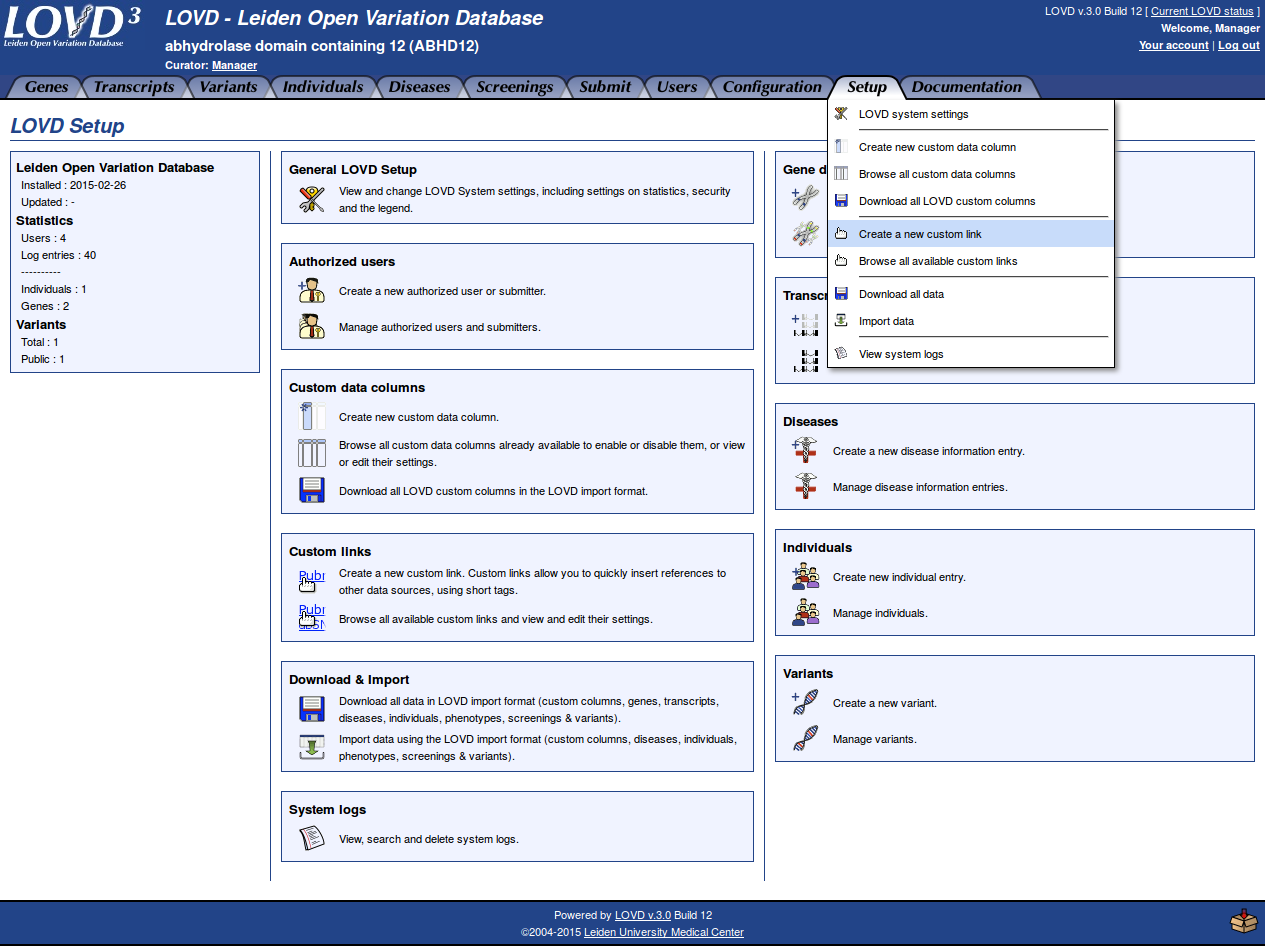
\includegraphics[width=\linewidth]
			 	 {/create_gene/create_link_I.png}};
				\begin{scope}[x={(image.south east)},y={(image.north west)}]
				  \draw[red,ultra thick,rounded corners] (0.65,0.71) rectangle (0.85,0.74);
					\draw[<-, >=latex, \pointercolor, line width=\pointerwidth] (0.65,0.725) to node[black]{A} (0.55,0.725);
				  \draw[red,ultra thick,rounded corners] (0.65,0.74) rectangle (0.85,0.77);
					\draw[<-, >=latex, \pointercolor, line width=\pointerwidth] (0.85,0.755) to node[black]{B} (0.95,0.755);
				  \draw[red,ultra thick,rounded corners] (0.22,0.32) rectangle (0.6,0.365);
					\draw[<-, >=latex, \pointercolor, line width=\pointerwidth] (0.22,0.3425) to node[black]{A} (0.12,0.3425);
				  \draw[red,ultra thick,rounded corners] (0.22,0.365) rectangle (0.6,0.41);
					\draw[<-, >=latex, \pointercolor, line width=\pointerwidth] (0.6,0.3875) to node[black]{B} (0.7,0.3875);
					%\drawgrid %help grid when positioning the boxes and pointers
				\end{scope}
			\end{tikzpicture}}
		\caption{From the Setup area you can go to ``Browse all available custom links'' (A).
		LOVD has some predefined links: DbSNP, GenBank, OMIM, PubMed and DOI. 
		For the purpose of the course we removed the DOI custom link.\newline
		Now we will create a new custom link for DOIs. 
		Click on the ``Create a new custom link'' link from the Setup	drop down menu tab, 
		 or select ``Create a new custom link'' from the Setup area (B).}
	  \label{fig:create_link_I}
  \end{shaded}
\end{figure}

\begin{figure}[ht]
  \begin{shaded}
  	\frame{
			\begin{tikzpicture}
				\node[anchor=south west,inner sep=0] (image) at (0,0) {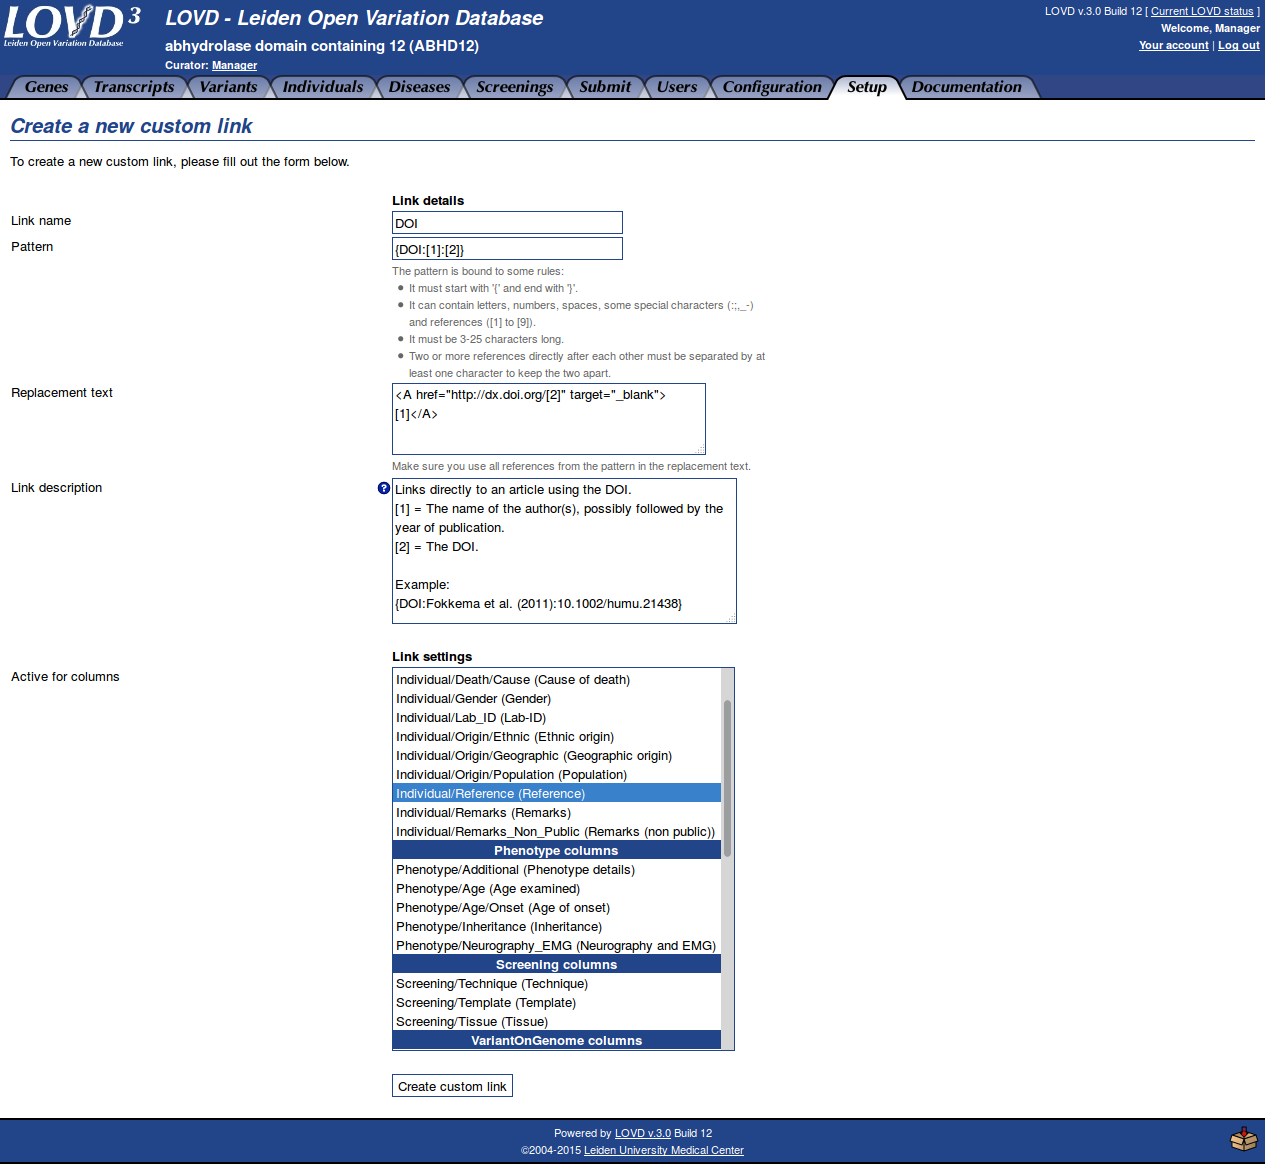
\includegraphics[width=\linewidth]
			 	 {/create_gene/create_link_II.png}};
				\begin{scope}[x={(image.south east)},y={(image.north west)}]
				  \draw[red,ultra thick,rounded corners] (0.3,0.77) rectangle (0.5,0.84);
					\draw[<-, >=latex, \pointercolor, line width=\pointerwidth] (0.5,0.805) to node[black]{A} (0.6,0.805);
				  \draw[red,ultra thick,rounded corners] (0.3,0.61) rectangle (0.56,0.67);
					\draw[<-, >=latex, \pointercolor, line width=\pointerwidth] (0.56,0.64) to node[black]{B} (0.66,0.64);
				  \draw[red,ultra thick,rounded corners] (0.3,0.46) rectangle (0.59,0.59);
					\draw[<-, >=latex, \pointercolor, line width=\pointerwidth] (0.59,0.525) to node[black]{C} (0.69,0.525);
				  \draw[red,ultra thick,rounded corners] (0.3,0.28) rectangle (0.59,0.445);
					\draw[<-, >=latex, \pointercolor, line width=\pointerwidth] (0.59,0.3625) to node[black]{D} (0.69,0.3625);
					%\drawgrid %help grid when positioning the boxes and pointers
				\end{scope}
			\end{tikzpicture}}
		\caption{Choose a name and pattern that curators need to use for LOVD to recognize the custom link (A). 
		Enter the (HTML enabled) text that should replace the entire pattern (B). 
		You need to use the same number of references that you used in the pattern.\newline
		Provide a short description about this link (C).
		Select the columns for which you want this custom link to be activated (D).\newline
		When you are ready, click ``Create custom link''.}
	  \label{fig:create_link_II}
  \end{shaded}
\end{figure}










\chapter{Creating and managing users}
The objective of this chapter is:
\begin{enumerate}
	\item 
	Create new user.
	\item 
	Manage user.
	\item 
	Make user curator.
\end{enumerate}
\label{chap:create_manage_users}





\section{Create users}
\begin{figure}[ht]
  \begin{shaded}
  	\frame{
			\begin{tikzpicture}
				\node[anchor=south west,inner sep=0] (image) at (0,0) {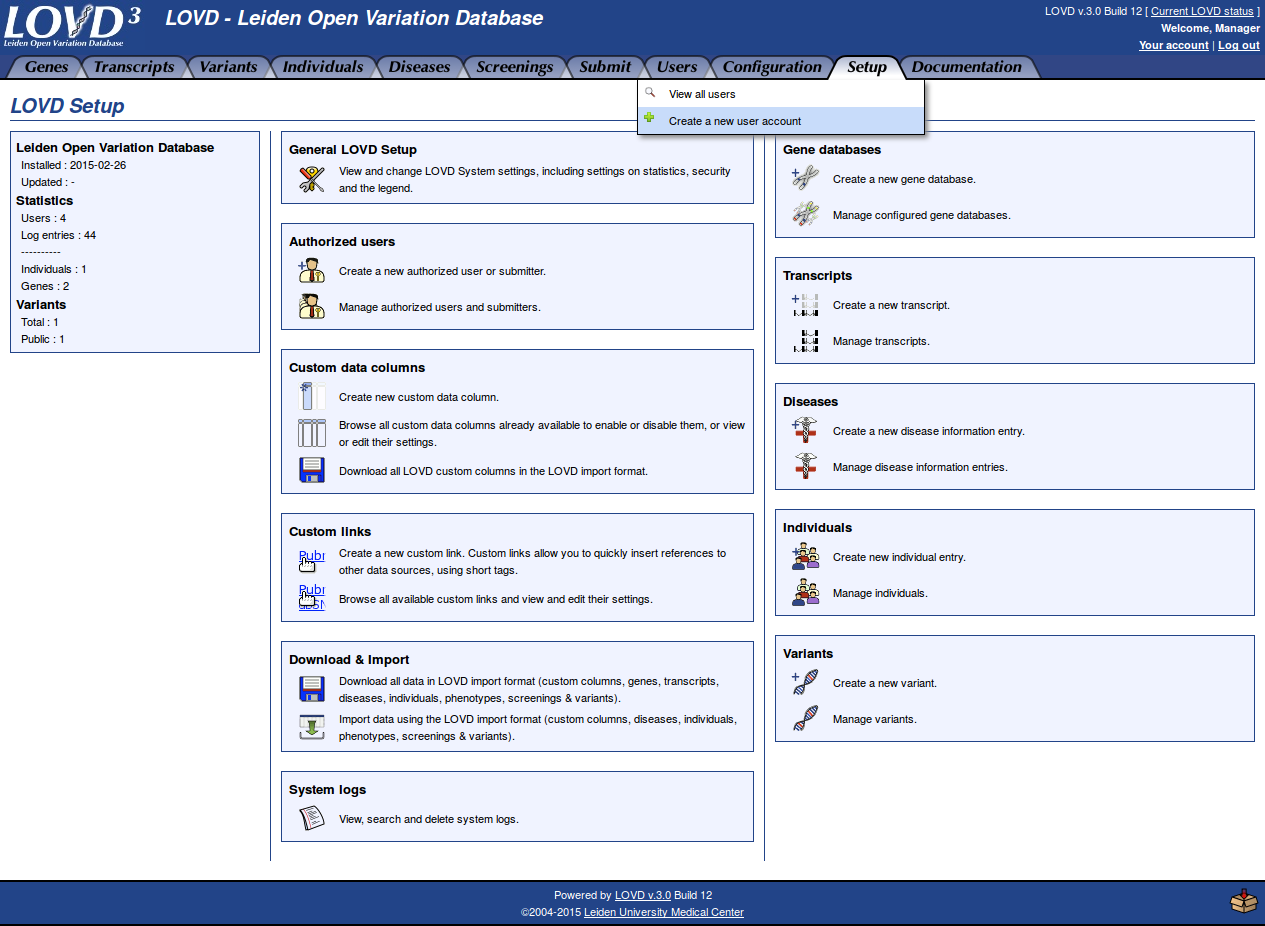
\includegraphics[width=\linewidth]
			 	 {/create_gene/create_user_I.png}};
				\begin{scope}[x={(image.south east)},y={(image.north west)}]
				  \draw[red,ultra thick,rounded corners] (0.22,0.69) rectangle (0.45,0.73);
					\draw[<-, >=latex, \pointercolor, line width=\pointerwidth] (0.45,0.71) to node[black]{A} (0.55,0.71);
				  \draw[red,ultra thick,rounded corners] (0.5,0.85) rectangle (0.65,0.88);
					\draw[<-, >=latex, \pointercolor, line width=\pointerwidth] (0.65,0.865) to node[black]{B} (0.75,0.865);
					%\drawgrid %help grid when positioning the boxes and pointers
				\end{scope}
			\end{tikzpicture}}
	  \caption{You can create a new user via ``Create a new authorized user or submitter'' from the Setup area (A).
	  Alternative: Use the ``Create new a user account'' link from the User drop down menu tab (B).}
  	\label{fig:create_user_I}
  \end{shaded}
\end{figure}

\begin{figure}[ht]
  \begin{shaded}
  	\frame{
			\begin{tikzpicture}
				\node[anchor=south west,inner sep=0] (image) at (0,0) {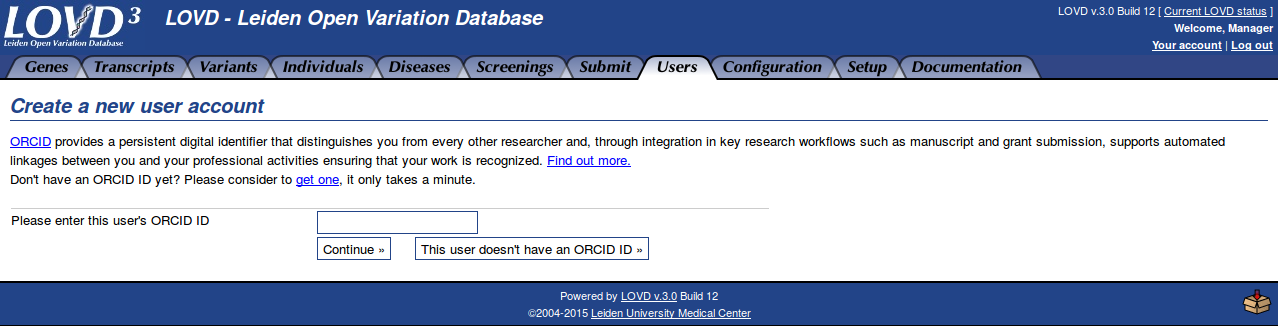
\includegraphics[width=\linewidth]
			 	 {/create_gene/create_user_III.png}};
				\begin{scope}[x={(image.south east)},y={(image.north west)}]
					%\draw[red,ultra thick,rounded corners] (0.01,0.38) rectangle (0.53,0.46);
					%\draw[<-, >=latex, \pointercolor, line width=\pointerwidth] (0.53,0.42) to node[black]{} (0.63,0.42);
					%\drawgrid %help grid when positioning the boxes and pointers
				\end{scope}
			\end{tikzpicture}}
		\caption{You can use individual's ORCID ID to create a new user, but this is not mandatory.
		Click ``This user doesn't have an ORCID ID'' if you do not want to use an ORCID ID.}
		\label{fig:create_user_III}
  \end{shaded}
\end{figure}

\begin{figure}[ht]
  \begin{shaded}
  	\frame{
			\begin{tikzpicture}
				\node[anchor=south west,inner sep=0] (image) at (0,0) {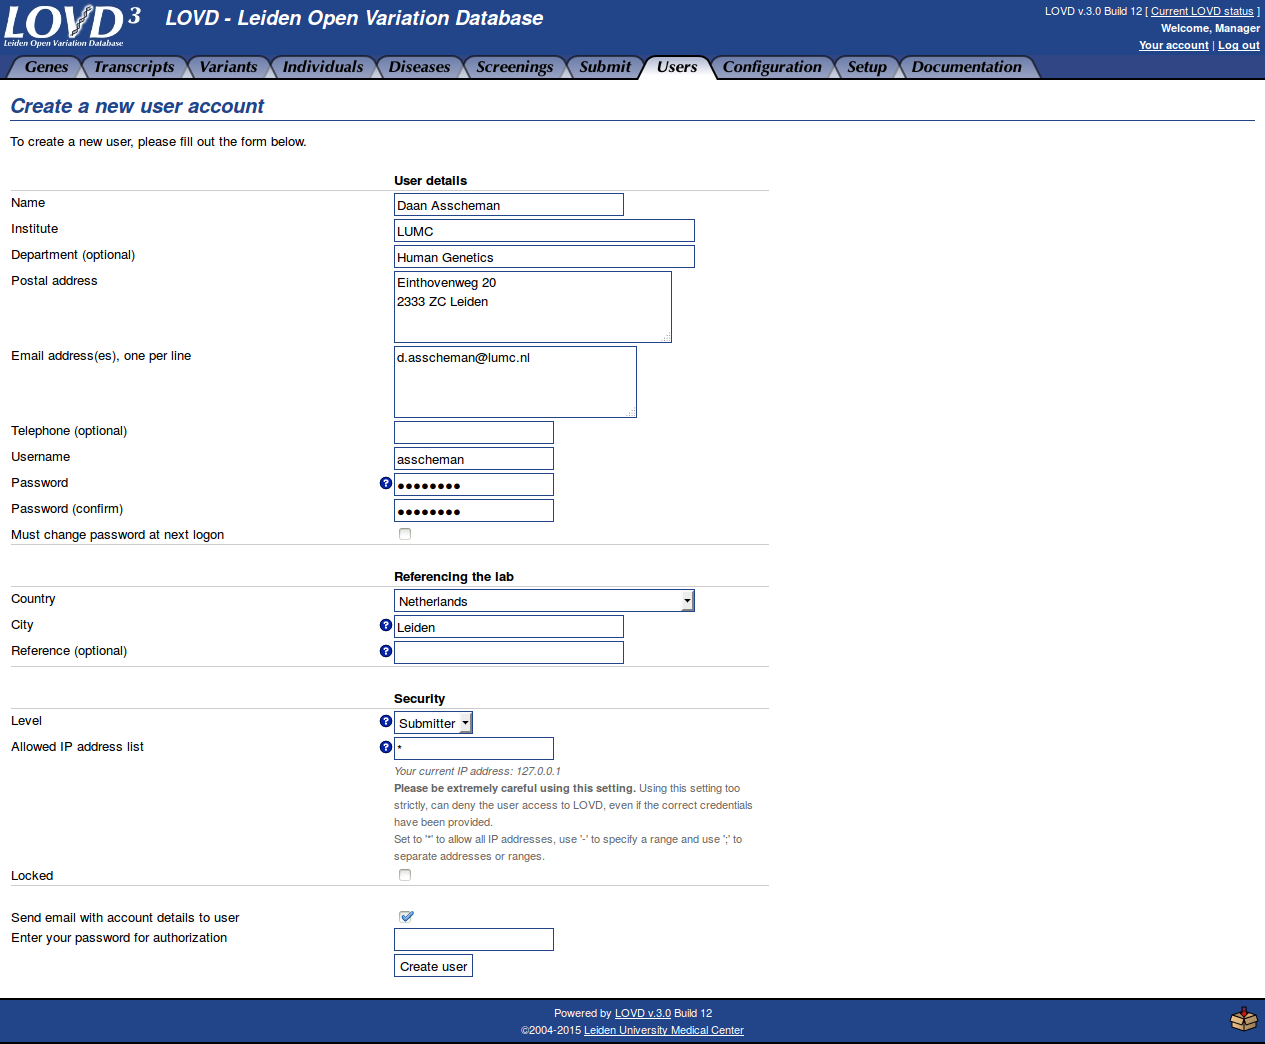
\includegraphics[width=\linewidth]
			 	 {/create_gene/create_user_IV.png}};
				\begin{scope}[x={(image.south east)},y={(image.north west)}]
				  %\draw[red,ultra thick,rounded corners] (0.01,0.38) rectangle (0.53,0.46);
					%\draw[<-, >=latex, \pointercolor, line width=\pointerwidth] (0.53,0.42) to node[black]{} (0.63,0.42);
					%\drawgrid %help grid when positioning the boxes and pointers
				\end{scope}
			\end{tikzpicture}}
		\caption{Enter the credentials of the new user and confirm with your password.}
		\label{fig:create_user_IV}
  \end{shaded}
\end{figure}
\clearpage





\section{Manage users}
\begin{figure}[ht]
  \begin{shaded}
  	\frame{
			\begin{tikzpicture}
				\node[anchor=south west,inner sep=0] (image) at (0,0) {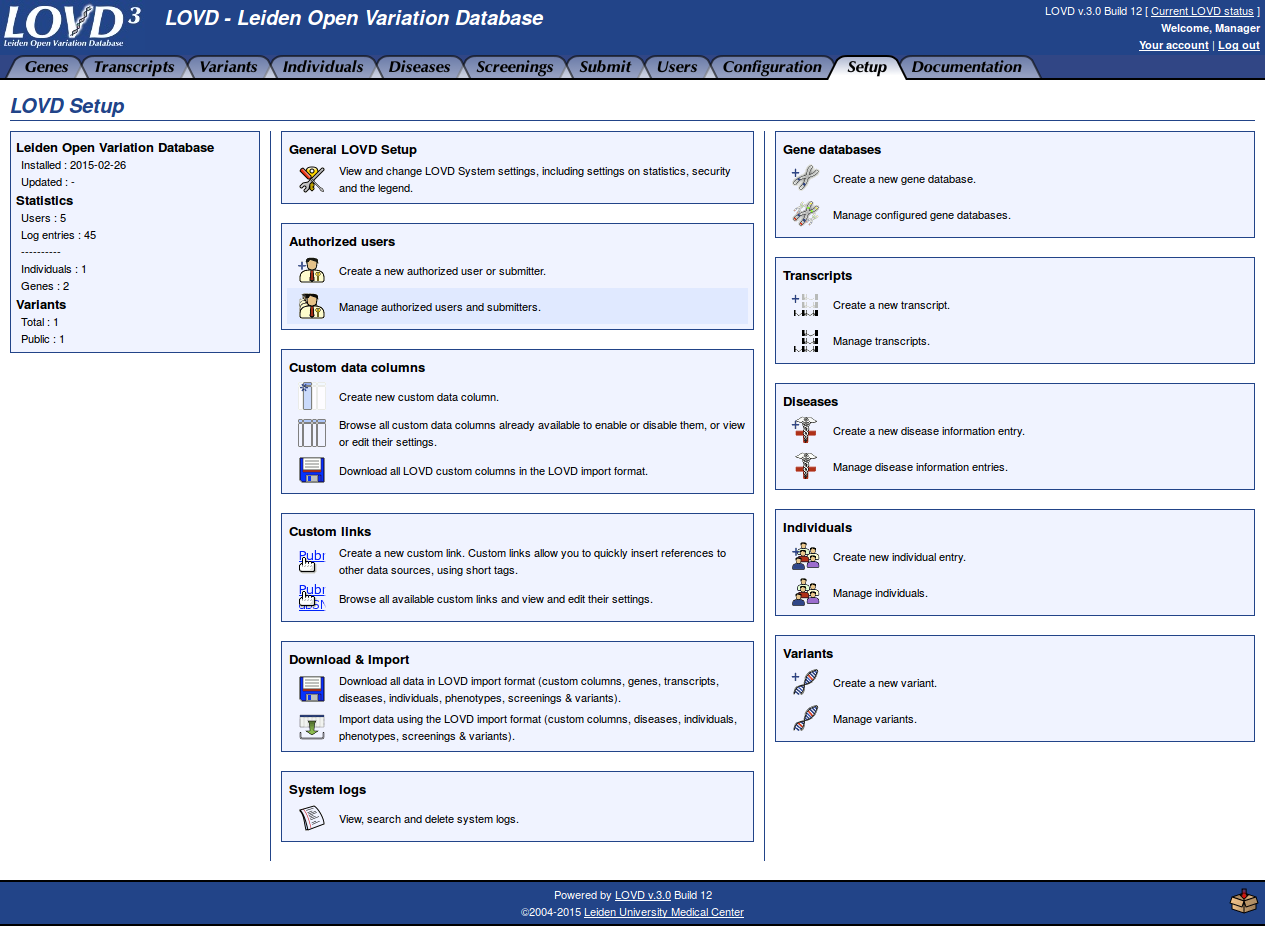
\includegraphics[width=\linewidth]
			 	 {/create_gene/manage_user_I.png}};
				\begin{scope}[x={(image.south east)},y={(image.north west)}]
				  \draw[red,ultra thick,rounded corners] (0.5,0.91) rectangle (0.57,0.94);
					\draw[<-, >=latex, \pointercolor, line width=\pointerwidth] (0.57,0.925) to node[black]{B} (0.67,0.925);
				 	\draw[red,ultra thick,rounded corners] (0.23,0.65) rectangle (0.46,0.69);
					\draw[<-, >=latex, \pointercolor, line width=\pointerwidth] (0.46,0.655) to node[black]{A} (0.56,0.655);
					%\drawgrid %help grid when positioning the boxes and pointers
				\end{scope}
			\end{tikzpicture}}
  	\caption{You can edit a user via ``Manage authorized users and submitters'' from the Setup area (A).
	  Or click the Users menu tab (B).}
  	\label{fig:manage_user_I}
  \end{shaded}
\end{figure}

\begin{figure}[ht]
  \begin{shaded}
  	\frame{
			\begin{tikzpicture}
				\node[anchor=south west,inner sep=0] (image) at (0,0) {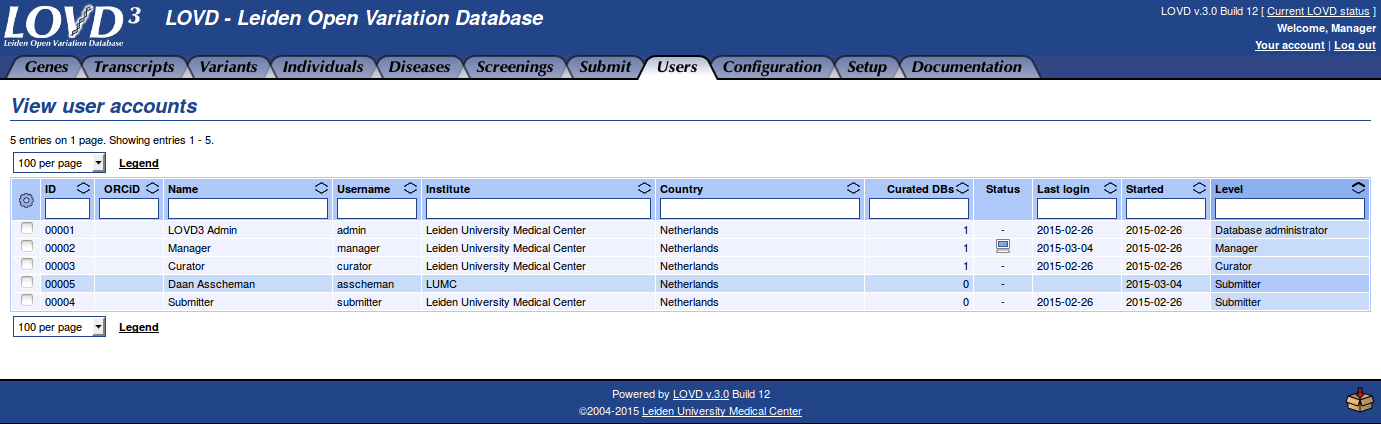
\includegraphics[width=\linewidth]
			 	 {/create_gene/manage_user_II.png}};
				\begin{scope}[x={(image.south east)},y={(image.north west)}]
				  \draw[red,ultra thick,rounded corners] (0.01,0.3) rectangle (0.6,0.36);
					\draw[<-, >=latex, \pointercolor, line width=\pointerwidth] (0.6,0.33) to node[black]{} (0.7,0.33);
					%\drawgrid %help grid when positioning the boxes and pointers
				\end{scope}
			\end{tikzpicture}}
  	\caption{Click on the user you want to edit.}
  	\label{fig:manage_user_II}
  \end{shaded}
\end{figure}

\begin{figure}[ht]
  \begin{shaded}
  	\frame{
			\begin{tikzpicture}
				\node[anchor=south west,inner sep=0] (image) at (0,0) {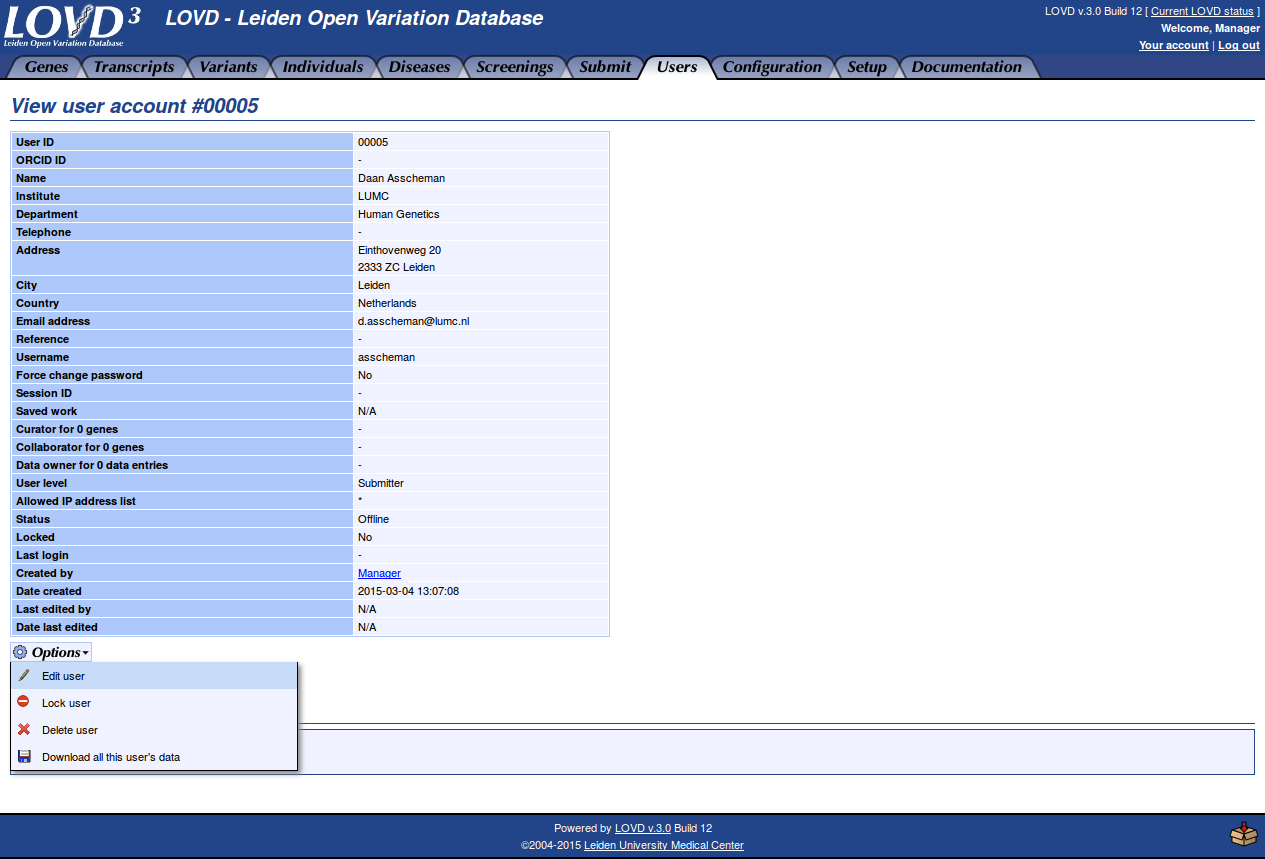
\includegraphics[width=\linewidth]
			 	 {/create_gene/manage_user_III.png}};
				\begin{scope}[x={(image.south east)},y={(image.north west)}]
				  \draw[red,ultra thick,rounded corners] (0.005,0.195) rectangle (0.15,0.26);
					\draw[<-, >=latex, \pointercolor, line width=\pointerwidth] (0.15,0.23) to node[black]{} (0.25,0.23);
					%\drawgrid %help grid when positioning the boxes and pointers
				\end{scope}
			\end{tikzpicture}}
		\caption{Click the Options drop down menu and select ``Edit user''. 
		You will go to the form ``Edit user'', this form is similar to the form ``Create user account'', see figure 
		 \ref{fig:create_user_IV}.}
		\label{fig:manage_user_III}
  \end{shaded}
\end{figure}
\clearpage




\section{Make user curator}
\begin{figure}[ht]
  \begin{shaded}
  	\frame{
			\begin{tikzpicture}
				\node[anchor=south west,inner sep=0] (image) at (0,0) {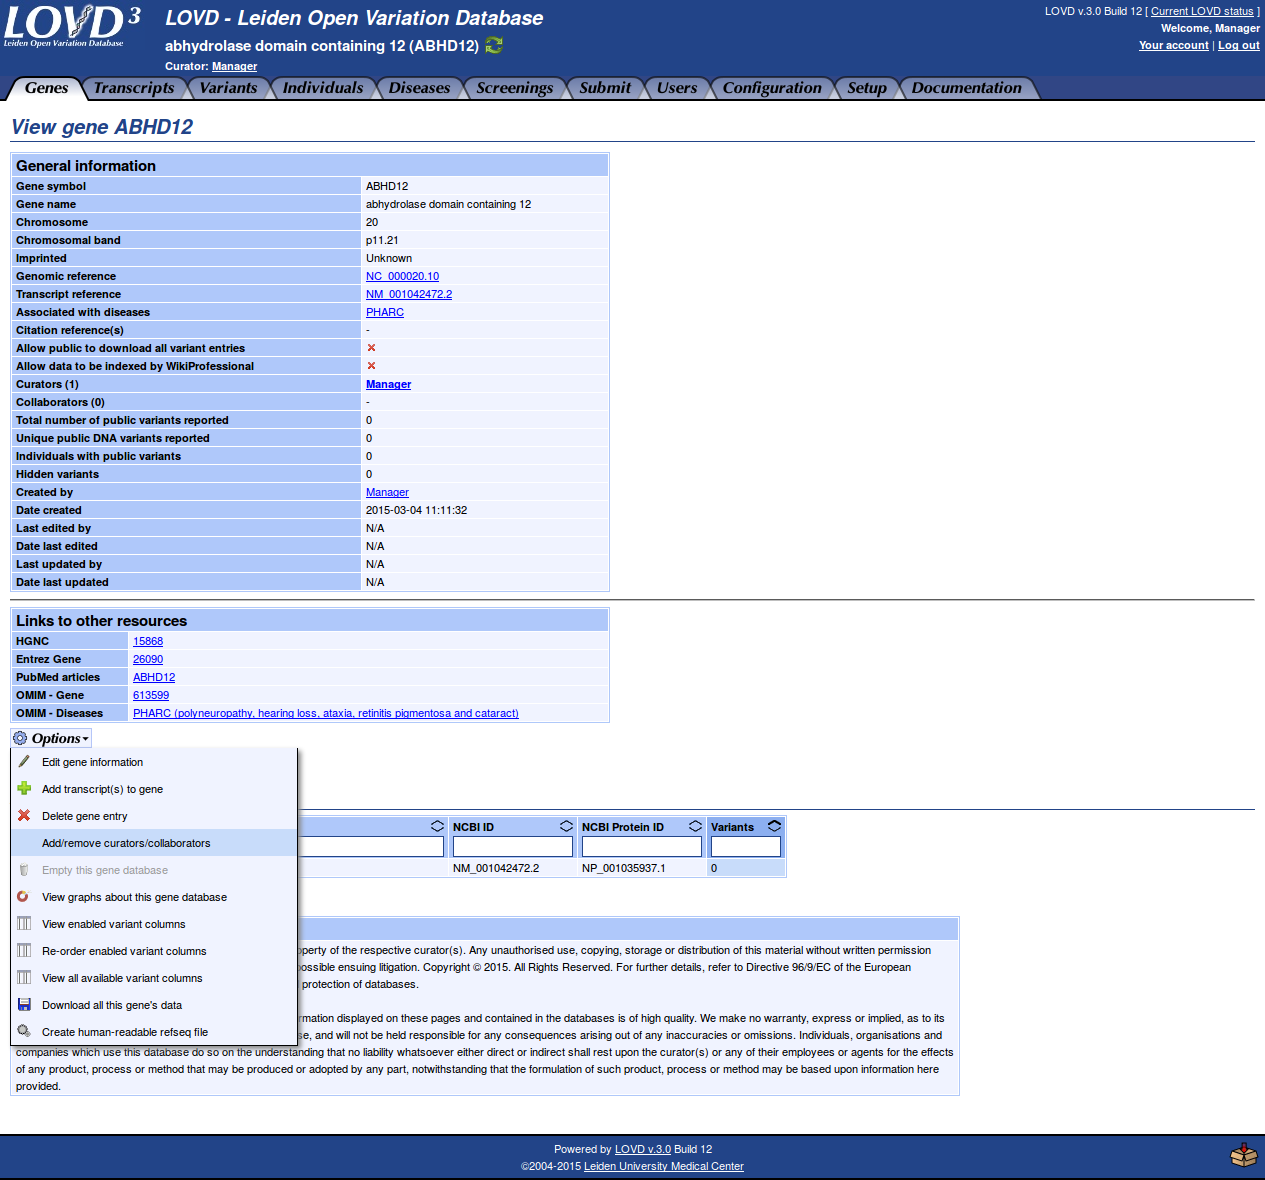
\includegraphics[width=\linewidth]
			 	 {/create_gene/make_user_curator_I.png}};
				\begin{scope}[x={(image.south east)},y={(image.north west)}]
				  \draw[red,ultra thick,rounded corners] (0.01,0.665) rectangle (0.36,0.685);
					\draw[<-, >=latex, \pointercolor, line width=\pointerwidth] (0.36,0.675) to node[black]{A} (0.46,0.675);
				  \draw[red,ultra thick,rounded corners] (0.01,0.27) rectangle (0.2,0.295);
					\draw[<-, >=latex, \pointercolor, line width=\pointerwidth] (0.2,0.2825) to node[black]{B} (0.3,0.2825);
					%\drawgrid %help grid when positioning the boxes and pointers
				\end{scope}
			\end{tikzpicture}}
  	\caption{On the ``View gene'' page you can see who curator is for a gene (A), in our example this is only 
  	 the manager.\newline
  	We will make our new user curator for the ABHD12 gene. 
  	Click on ``Add/remove curators/collaborators''(B).}
  	\label{fig:make_user_curator_I}
  \end{shaded}
\end{figure}

\begin{figure}[ht]
  \begin{shaded}
  	\frame{
			\begin{tikzpicture}
				\node[anchor=south west,inner sep=0] (image) at (0,0) {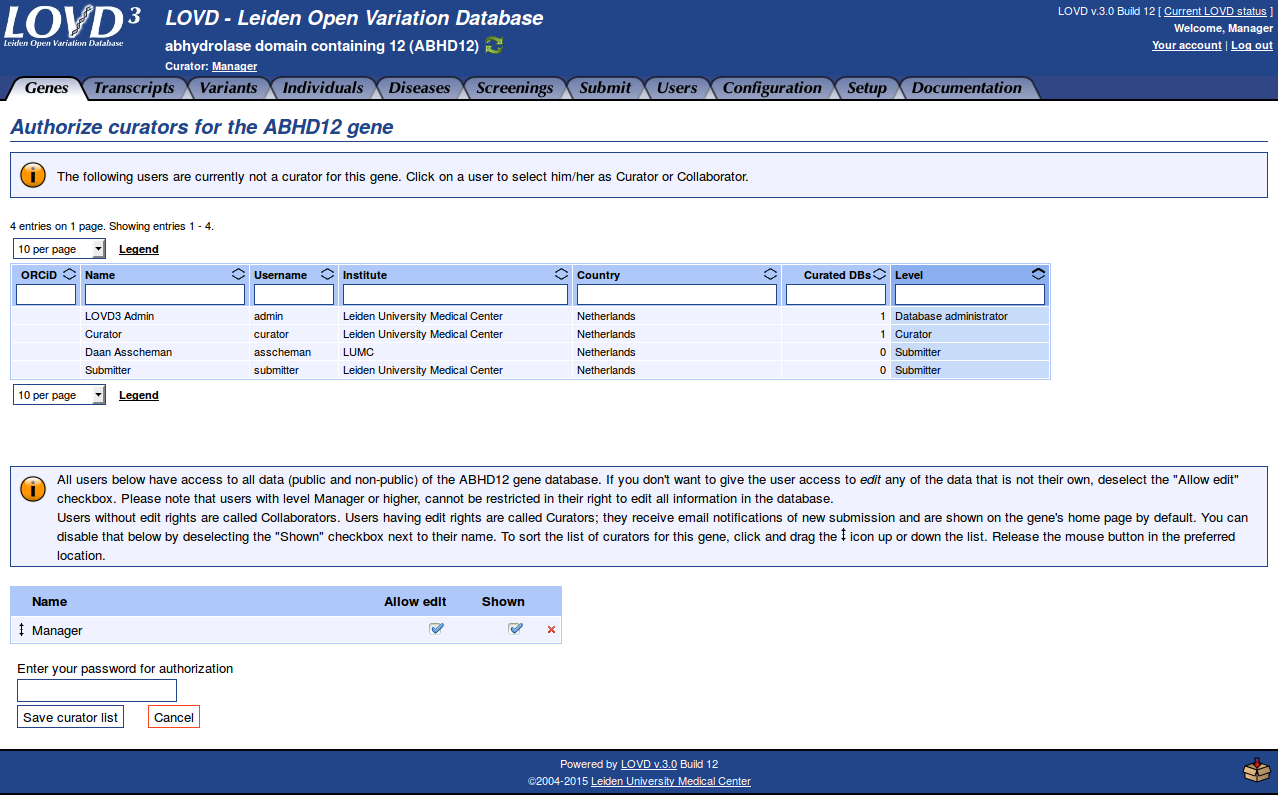
\includegraphics[width=\linewidth]
			 	 {/create_gene/make_user_curator_II.png}};
				\begin{scope}[x={(image.south east)},y={(image.north west)}]
				  \draw[red,ultra thick,rounded corners] (0.01,0.544) rectangle (0.56,0.574);
					\draw[<-, >=latex, \pointercolor, line width=\pointerwidth] (0.56,0.559) to node[black]{} (0.66,0.559);
					%\drawgrid %help grid when positioning the boxes and pointers
				\end{scope}
			\end{tikzpicture}}
  	\caption{Click the user you want to add as a curator.}
	  \label{fig:make_user_curator_II}
  \end{shaded}
\end{figure}

\begin{figure}[ht]
  \begin{shaded}
  	\frame{
			\begin{tikzpicture}
				\node[anchor=south west,inner sep=0] (image) at (0,0) {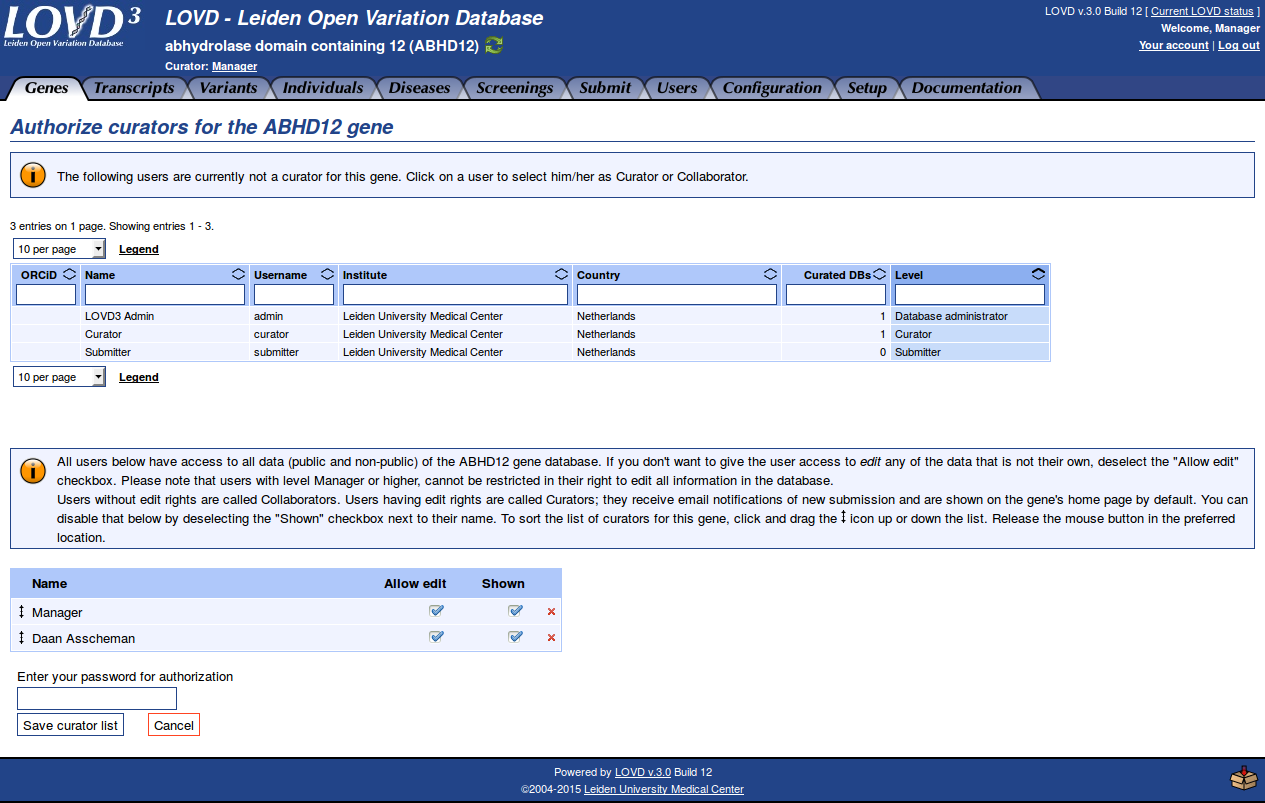
\includegraphics[width=\linewidth]
			 	 {/create_gene/make_user_curator_III.png}};
				\begin{scope}[x={(image.south east)},y={(image.north west)}]
				  \draw[red,ultra thick,rounded corners] (0.01,0.19) rectangle (0.46,0.22);
					\draw[<-, >=latex, \pointercolor, line width=\pointerwidth] (0.46,0.205) to node[black]{} (0.56,0.205);
					%\drawgrid %help grid when positioning the boxes and pointers
				\end{scope}
			\end{tikzpicture}}
  	\caption{The user will appear in the list of curators.
  	You can make the user a collaborator by unchecking the ``Allow edit'' field, 
  	 the user can still see all public and unpublic data in this gene database, but they can't edit it,
  	 like curators can.\newline 
		The ``Shown'' checkbox indicates whether or not the user's name and email address is shown
		 on the gene homepage and on the top of every page while this gene is selected.\newline
		To remove an user as a curator or collaborator, click the red cross at the far right side of the table.
  	Confirm with your password.}
	  \label{fig:make_user_curator_III}
  \end{shaded}
\end{figure}

\begin{figure}[ht]
  \begin{shaded}
  	\frame{
			\begin{tikzpicture}
				\node[anchor=south west,inner sep=0] (image) at (0,0) {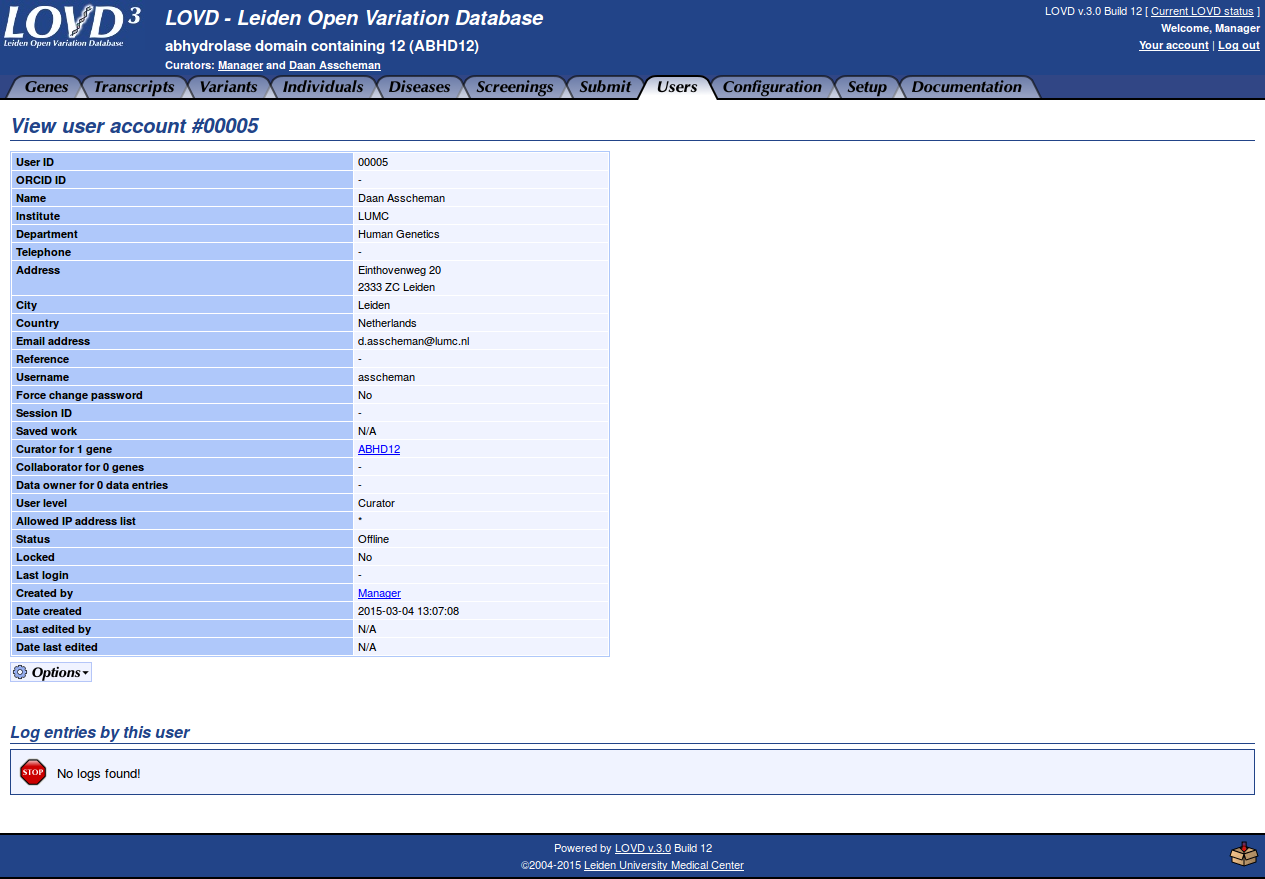
\includegraphics[width=\linewidth]
			 	 {/create_gene/make_user_curator_IV.png}};
				\begin{scope}[x={(image.south east)},y={(image.north west)}]
				  \draw[red,ultra thick,rounded corners] (0.005,0.478) rectangle (0.35,0.5);
					\draw[<-, >=latex, \pointercolor, line width=\pointerwidth] (0.35,0.489) to node[black]{} (0.45,0.489);
					%\drawgrid %help grid when positioning the boxes and pointers
				\end{scope}
			\end{tikzpicture}}
  	\caption{In the ``View user account'' you will see that the gene is added to ``Curator for''.}
	  \label{fig:make_user_curator_IV}
  \end{shaded}
\end{figure}

\begin{figure}[ht]
  \begin{shaded}
  	\frame{
			\begin{tikzpicture}
				\node[anchor=south west,inner sep=0] (image) at (0,0) {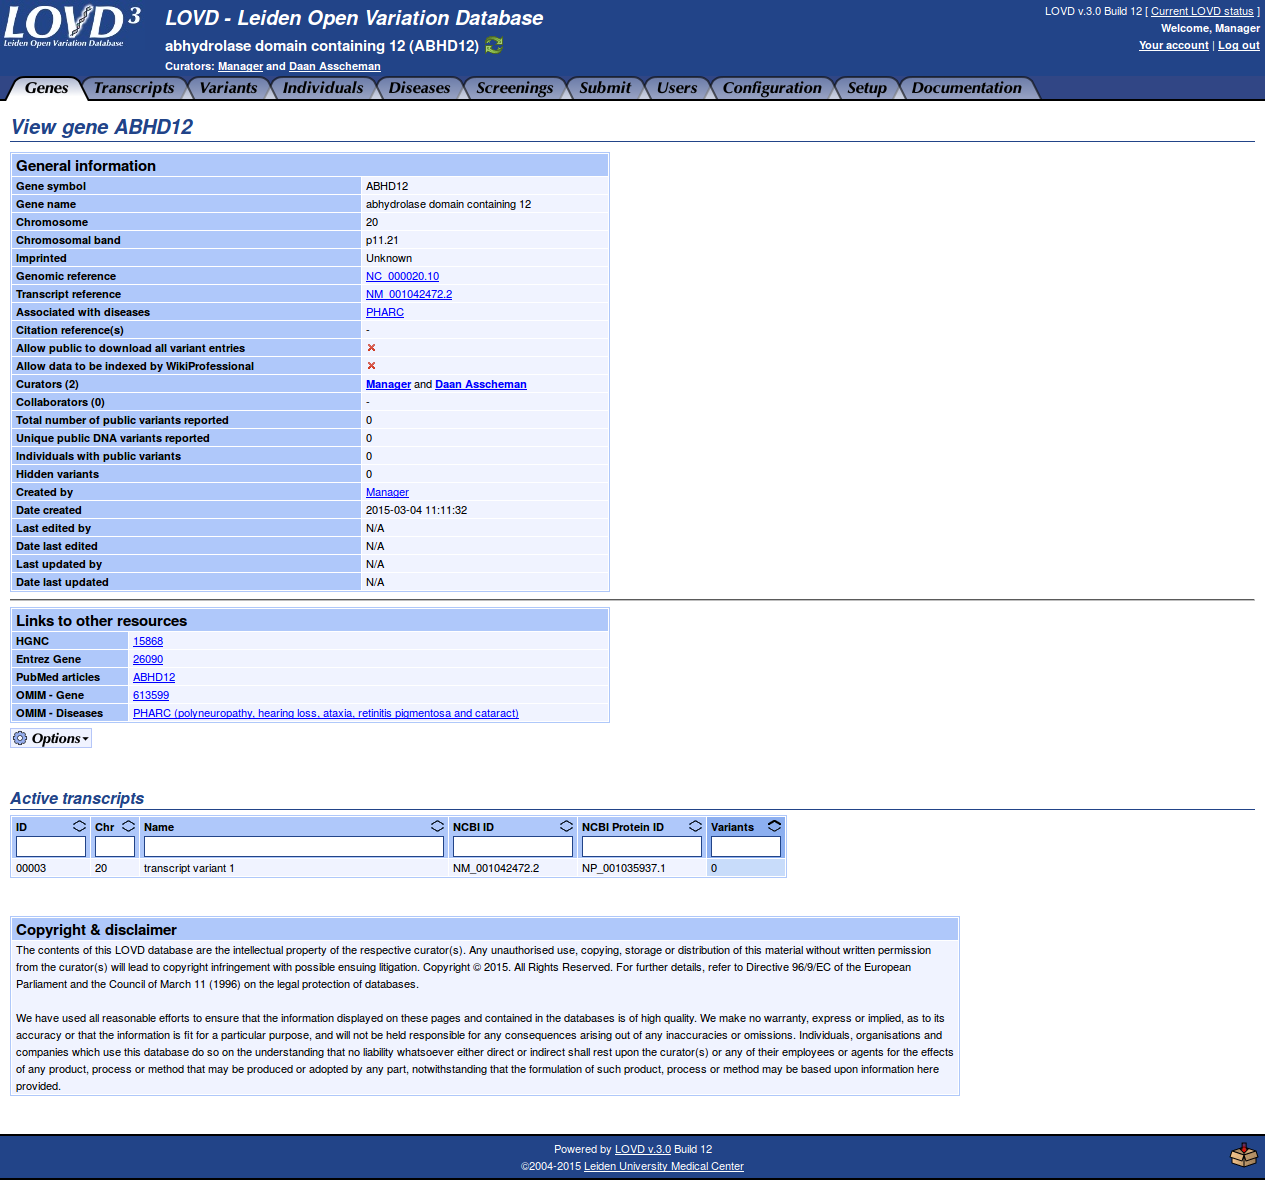
\includegraphics[width=\linewidth]
			 	 {/create_gene/make_user_curator_V.png}};
				\begin{scope}[x={(image.south east)},y={(image.north west)}]
				  \draw[red,ultra thick,rounded corners] (0.005,0.66) rectangle (0.44,0.69);
					\draw[<-, >=latex, \pointercolor, line width=\pointerwidth] (0.44,0.675) to node[black]{} (0.54,0.675);
					%\drawgrid %help grid when positioning the boxes and pointers
				\end{scope}
			\end{tikzpicture}}
  	\caption{In the ``View gene'' you can see that the user is added to Curators.}
	  \label{fig:make_user_curator_V}
  \end{shaded}
\end{figure}
\clearpage










\end{document}

%10
\chapter{}
%5
\section{}
%3
\subsection{}
%1
\subsubsection{}


%%%%%%%%%%%%%%%%%%%%%%%%%%%%%%%%%%%%%%%%%% NEW MAXIMUM LINE LENGTH (120 char) %%%%%%%%%%%%%%%%%%%%%%%%%%%%%%%%%%%%%%%%%%
